\documentclass[t]{beamer}

\usepackage[T1]{fontenc}
\usepackage[utf8]{inputenc}
\usepackage{upquote}

\newcommand{\titel}{Introduction to CMake}
\newcommand{\titelkurz}{Introduction to CMake}
\newcommand{\vortragender}{Raphael M\"unster}
\newcommand{\koautoren}{}
\newcommand{\ortdatum}{\today}

\usepackage{array}
\usepackage{ragged2e}

\usepackage[ngerman,english]{babel}
\usepackage[babel,german=quotes]{csquotes}
\usepackage{graphicx}
\usepackage{textpos}
\usepackage{tikz}

\usetikzlibrary{shapes.arrows,calc,decorations.pathmorphing}
\usetikzlibrary{arrows.meta,shapes.misc}
\usetikzlibrary{fit}

%%\usepackage{gitinfo}
\usepackage{showframe}
\usepackage{shadowtext}

\usetheme{-tud-4-3}

% Title page
\title[\titelkurz]{\titel}
\author{Raphael M\"unster}
\date{\ortdatum\\[-0.2cm]}
\institute{TU Dortmund}

% ------------------------------------------------------------------------------------
% VORTRAG ESCO 2012     FRIEDRICH-ALEXANDER-UNIVERSITAET ERLANGEN-NUERNBERG
% ------------------------------------------------------------------------------------
%     erstellt von Christopher Basting, 21. Juni 2012
% ------------------------------------------------------------------------------------
% abbrev.tex
% ------------------------------------------------------------------------------------

% Mathe spezifische Packages
\usepackage{amsmath,amsfonts}
\usepackage{dsfont}

\renewcommand{\d}{{\rm d}} % d fuer dx bei Ableitungen / Integralen
\newcommand{\gdw}{\Leftrightarrow} % <=>
\newcommand{\x}{\cdot}
\newcommand{\ma}{\left( \begin{array}{*{19}{c}}} % Matrix oeffnen
\newcommand{\me}{\end{array}\right)} % Matrix schliessen
\newcommand{\mA}{\left[ \begin{array}{*{19}{c}}} % Matrix oeffnen
\newcommand{\mE}{\end{array}\right]} % Matrix schliessen
\newcommand{\C}{\mathds{C}}
\newcommand{\E}{\mathds{1}}
\newcommand{\F}{\mathds{F}}
\newcommand{\K}{\mathds{K}}
\newcommand{\N}{\mathds{N}}
\newcommand{\Q}{\mathds{Q}}
\newcommand{\R}{\mathds{R}}
\newcommand{\Z}{\mathds{Z}}
\newcommand{\id}{\mathds{1}}
\renewcommand{\d}{\,{\rm d}}
\newcommand{\D}{{\rm D}}
\newcommand{\richtig}{\checkmark}
\newcommand{\falsch}{\lightning}
\newcommand{\ra}{\rightarrow}
\newcommand{\Ra}{\Rightarrow}
\newcommand{\la}{\leftarrow}
\newcommand{\La}{\Leftarrow}

\newcommand{\abbildung}[3]{#1 \, : \, #2 \rightarrow #3}
\newcommand{\grad}{\nabla}

%\renewcommand{\phi}{\varphi}
\newcommand{\cL}{\mathcal{L}}
\newcommand{\cO}{\mathcal{O}}

\newcommand{\eps}{\varepsilon}

\renewcommand{\vec}{\bold}
\newcommand{\dist}{{\rm dist}}

\newcommand{\mat}[1]{\textsf{\textbf{#1}}}

\usepackage{amscd,amssymb} 

\providecommand{\abs}[1]{\lvert#1\rvert}
\providecommand{\norm}[1]{\left\lVert#1\right\rVert}
\providecommand{\normNoAdjust}[1]{\lVert#1\rVert}
\providecommand{\transpose}[1]{{#1}^\top}
\providecommand{\inversetranspose}[1]{{#1}^{-\top}}



\shadowoffsetx{0.7pt}
\shadowoffsety{0.7pt}


\newcommand{\itemra}{\item[$\rightarrow$]}
%\newcommand{\TUgreen}{\color{TUgreen}}
\newcommand{\TUgreen}{\color{red}}
\usepackage{hyperref}

\usepackage{listings}

\lstset{breaklines=true,      % sets automatic line breaking
basicstyle=\ttfamily\LARGE,
language=TeX,
escapechar=@
}

\usepackage{fancybox, graphicx}

\usepackage{lmodern}

% Einige Befehle (s. Thomas Rohkaemper's Slides)
\definecolor{darkgray}{gray}{0.3}
\newcommand{\kommandozeile}[1]{{{\ttfamily\bfseries \color{white}\colorbox{black}{#1}}}}
\newcommand{\dateiname}[1]{{\ttfamily\bfseries \color{red}#1}}
\newcommand{\emphword}[1]{{\color{red}#1}}
\newcommand{\keyword}[1]{\texttt{\color{blue}#1}}
\newcommand{\emphkeyword}[1]{\texttt{\color{red}#1}}
\newcommand{\befehl}[1]{\texttt{\color{blue}\symbol{`\\}#1}}
\newcommand{\tabitem}{~~\llap{\color{red}\textbullet}~~}

\newcommand{\latexBeispielDatei}[2]{
	\begin{columns}[T]
		\begin{column}{0.54\textwidth}
			\begin{block}{#1}
				\lstinputlisting{#2.tex}
			\end{block}
		\end{column}
		\begin{column}{0.44\textwidth} \vspace{-2.5cm}
			\shadowbox{\includegraphics[width=0.9\textwidth]{#2.pdf}}
		\end{column}
	\end{columns}
}

\newcommand{\latexBeispielDateiCodeAnmerkungen}[3]{
	\begin{columns}[T]
		\begin{column}{0.54\textwidth}
			\begin{block}{#1}
				\lstinputlisting{#2.tex}
			\end{block}
		\end{column}
		\begin{column}{0.44\textwidth}
			#3
		\end{column}
	\end{columns}
}

\newcommand{\latexBeispielDateiKlein}[2]{
	\begin{columns}[T]
		\begin{column}{0.54\textwidth}
			\begin{block}{#1}
				\lstinputlisting[basicstyle=\ttfamily\large]{#2.tex}
			\end{block}
		\end{column}
		\begin{column}{0.44\textwidth} \vspace{-2.5cm}
			\shadowbox{\includegraphics[width=0.9\textwidth]{#2.pdf}}
		\end{column}
	\end{columns}
}


\newcommand{\latexBeispielDirekt}[2]{
	\begin{columns}[c]
		\begin{column}{0.54\textwidth}
			\begin{block}{#1}
			\lstinputlisting{#2}
			\end{block}
		\end{column}
		\begin{column}{0.44\textwidth}
			\shadowbox{\begin{minipage}{0.99\textwidth} \input{#2} \end{minipage}}
		\end{column}
	\end{columns}
}

\newcommand{\latexBeispielDirektKlein}[2]{
	\begin{columns}[c]
		\begin{column}{0.54\textwidth}
			\begin{block}{#1}
			\lstinputlisting[basicstyle=\ttfamily\large]{#2}
			\end{block}
		\end{column}
		\begin{column}{0.44\textwidth}
			\shadowbox{\begin{minipage}{0.99\textwidth} \input{#2} \end{minipage}}
		\end{column}
	\end{columns}
}

\newcommand{\latexBeispielDirektFake}[3]{
	\begin{columns}[c]
		\begin{column}{0.54\textwidth}
			\begin{block}{#1}
			\lstinputlisting{#2}
			\end{block}
		\end{column}
		\begin{column}{0.44\textwidth}
			\shadowbox{\begin{minipage}{0.99\textwidth} #3 \end{minipage}}
		\end{column}
	\end{columns}
}

\begin{document}

%
%
%%%%%%%%%%%%%%%%%%%%%%%%%%%%%%%%%%%%%%%%%%%%%%%%%%%%%%%%%%%%%%%%%%%%%%%%%%%%%
%
%
% Kopf- und Fußzeile abschalten
\frame[plain,c]{\titlepage}

% ab jetzt Autoren ohne Unterstreichung des Vortragenden
\author{\vortragender}

% keine eigene Seite für jede Section einblenden (kann mit \activateOwnSectionPage rückgängig gemacht werden)
\deactivateOwnSectionPage 


%%%%%%%%%%%%%%%%%%%%%%%%%%%%%%%%%%%%%%%%%%%%%%%%%%%%%%%%%%%%%%%%%%%%%%%%%%%%%
% N O R M A L E   U N I - V E R S I O N
%%%%%%%%%%%%%%%%%%%%%%%%%%%%%%%%%%%%%%%%%%%%%%%%%%%%%%%%%%%%%%%%%%%%%%%%%%%%%
\begin{frame}
	\frametitle{Slides and Examples}

        \begin{itemize}
		\item Slides:\\
                  \url{https://depot.tu-dortmund.de/dlep3}
		\item Examples:\\ 
                  \url{https://depot.tu-dortmund.de/5al36} 
        \end{itemize}

\end{frame}

\begin{frame}
	\frametitle{About ParaView}

      \begin{block}{ParaView Features}
        \begin{itemize}
		\item Open-source and multi-platfrom visualization software
		\item Visualization backend provided by VTK library
		\item Huge number of visualization filters  
                \item Extension is possible by programmable filters (Python) or 
                \item User defined plugins  
		\item Import and export of data to various formats used in CFD packages
		\item Easy access to numerical data for internal or external plotting etc.
		\item Tasks can be automated by using the PvPython interface
		\item Client/Server paradigm to view Big Data on remote clusters
        \end{itemize}
      \end{block}

\end{frame}


\begin{frame}
  \frametitle{ParaView Software Ecosystem}
  \vspace{-0.9cm}
  \begin{tikzpicture}[remember picture,overlay]
    \tikzset{shift={(current page.center)},yshift=-1.5cm}

    \node[text width=8cm] (C1) at (-8, -0.0) {
      \begin{block}{VTK}
        \begin{itemize}
          \item Visualization backend
          \item Uses OpenGL
        \end{itemize}
      \end{block}
    };

    \node[text width=8cm] (C2) at (8,-0.7) {
      \begin{block}{Qt (cute)}
        \begin{itemize}
          \item Provides widges and other GUI controls
          \item Support for modular plugins
        \end{itemize}
      \end{block}
    };

    \node[text width=8cm] (C3) at (0,4) {
      \begin{block}{CMake}
        \begin{itemize}
          \item Script language to control the building process
          \item Generates a wide range of specific build files
        \end{itemize}
      \end{block}
    };

    \node[text width=8cm] (C4) at (0,-4.85) {
      \begin{block}{ParaView}
        \begin{itemize}
          \item VTK visualization by GUI
          \item Scripting via Python
          \item Extension by plugins
        \end{itemize}
      \end{block}
    };

\end{tikzpicture}
\end{frame}


\begin{frame}
  \frametitle{Use Cases of Visualization Software}

      \begin{block}{Typical ParaView Use Cases}
        \begin{itemize}
          \item Provide an intuitive illustration of raw simulation data

          \item Highlight key features of specific flow features

          \item Provide an intuitive understanding for non-expert viewers  

          \item Help in the testing/debugging process of CFD software 

          \item Assist during result validation by providing analysis tools  

          \item Convert data in different formats in order to communicate with scientific partners
        \end{itemize}
      \end{block}

\end{frame}

\begin{frame}
  \frametitle{ParaView Interface}

  \begin{tikzpicture}[remember picture,overlay]
    \tikzset{shift={(current page.center)},yshift=-1.5cm}

    \node[align=center,scale=0.3,transform shape] (C1) at (0,0)
    {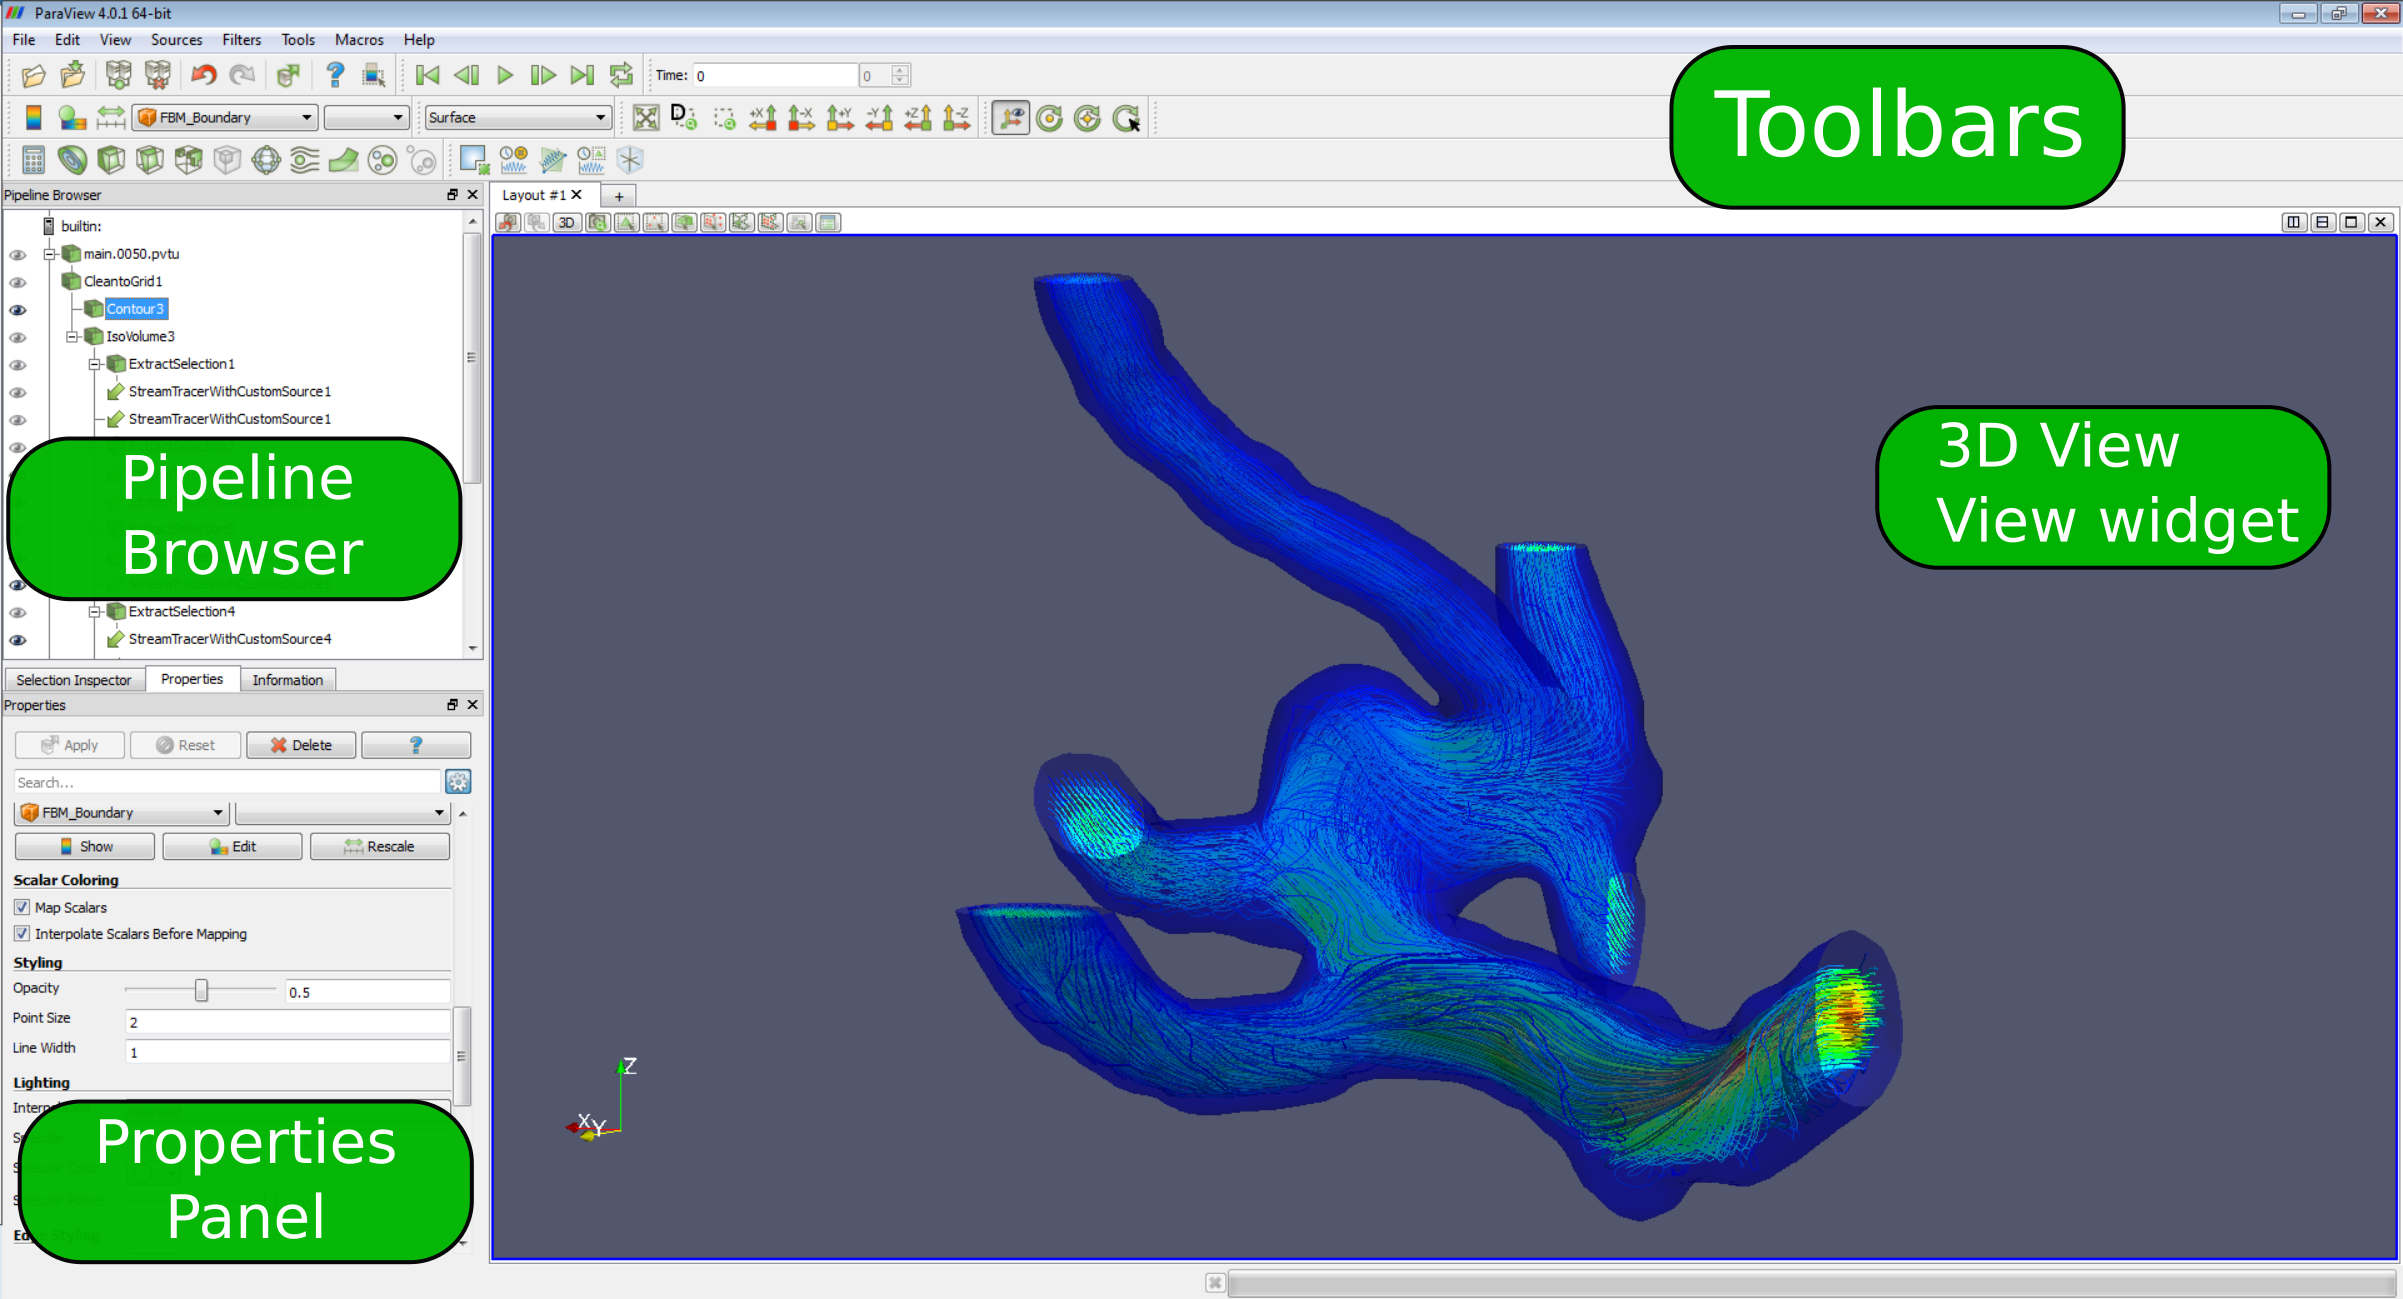
\includegraphics{screenshots/pv-gui.png}};

\end{tikzpicture}

\end{frame}

\begin{frame}[fragile]
  \frametitle{Filter Pipeline Concept}

    \begin{minipage}{0.45 \textwidth}

      \begin{tikzpicture}%[nodes=draw]

    \node[text width=8cm] (C1) at (-8, 1.25) {
      \begin{block}{Filter Pipeline}
        \begin{itemize}
          \item A \keyword{filter} is an operation on an input data set
          \item Filters can be chained (pipelined)  
          \item More complex visualizations require multiple filters 
        \end{itemize}
      \end{block}
    };

    \node[align=center,scale=0.5,transform shape] (C1) at (-10,-5.0)
    {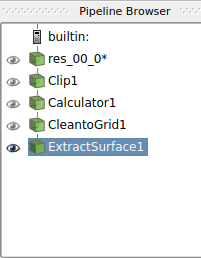
\includegraphics{screenshots/filters.png}};

    \end{tikzpicture}

    \end{minipage}
    \begin{minipage}{0.45 \textwidth}
      \begin{center}
        \begin{tikzpicture}%[nodes=draw]

          \node[align=center,scale=0.189,transform shape] (C1) at (10,-1)
          {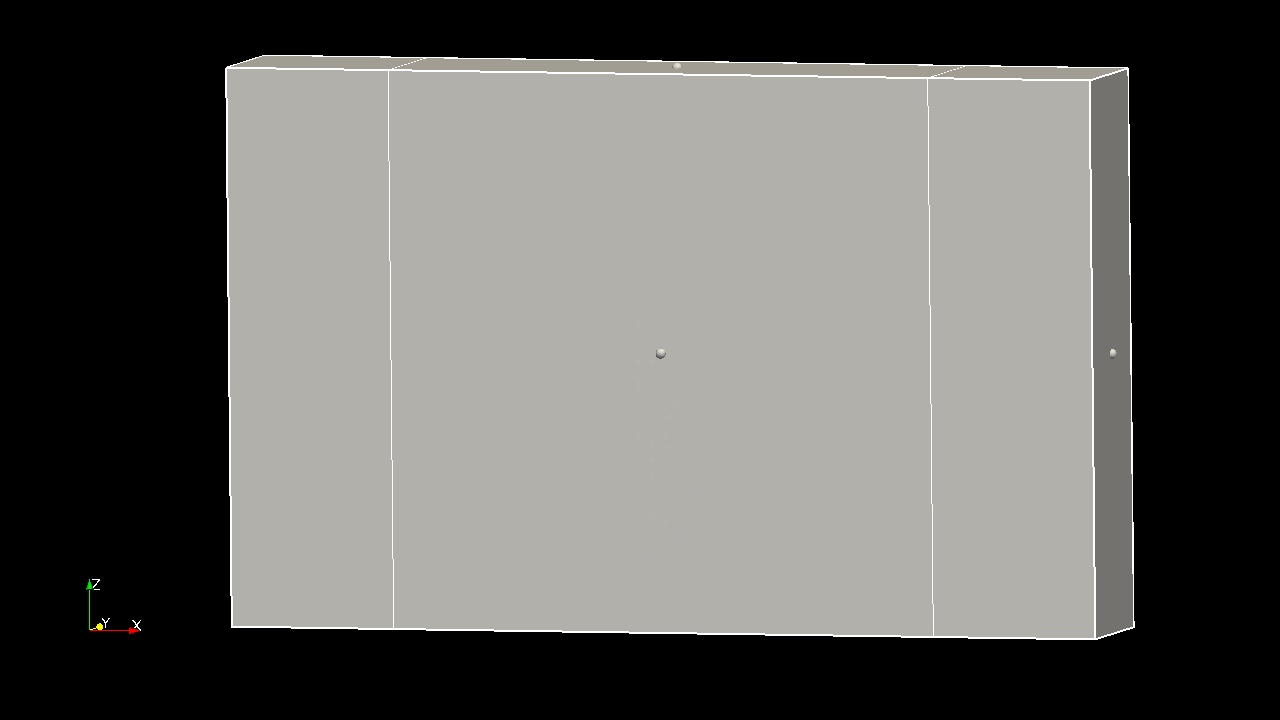
\includegraphics{screenshots/begin-filter.png}};

            \node [scale=2.8,
            fill=TUgreen, 
            single arrow,
            rotate=270, 
            font=\sffamily
            ] at (10.0,-4.22)  
            {\rotatebox{270}{}};

          \node[align=center,scale=0.8,transform shape] (C2) at (10,-8)
          {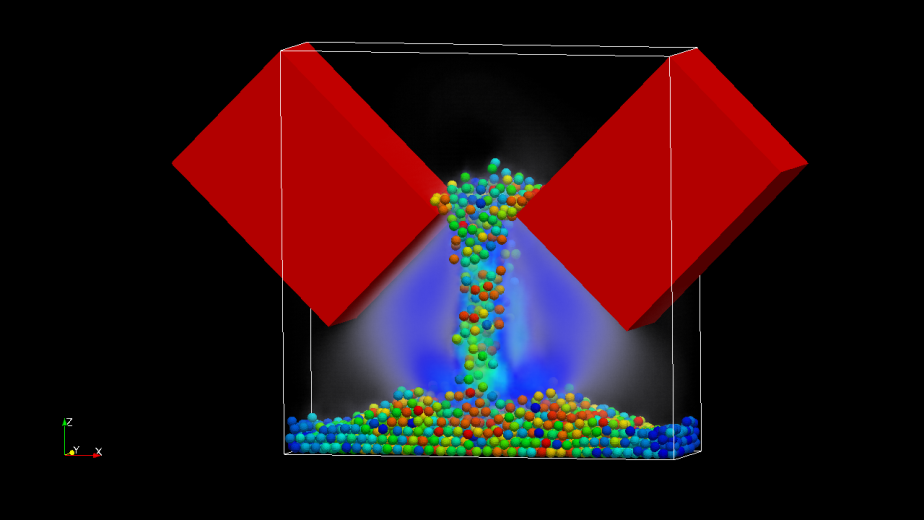
\includegraphics{screenshots/end-filter.png}};

        \end{tikzpicture}
      \end{center}
    \end{minipage}
\end{frame}

\begin{frame}
  \frametitle{Camera and Axes Toolbar}

  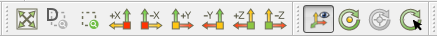
\includegraphics[width=\textwidth]{screenshots/camerabar.png}

    \begin{itemize}
      \item Reset the camera to its default parameters
      \item Magnify a rectangular selection of the view area
      \item Choose a certain coordinate axes plane to look at
      \item Toggle rendering of orientation axes 
      \item Toggle rendering of center of rotation 
      \item Select a new center of rotation 
    \end{itemize}
\end{frame}

\begin{frame}
  \frametitle{Basic Filters}

    \begin{itemize}
      \item \keyword{Slice}: Extract a plane, box-, sphere- or cylinder surface out of a data set
      \item \keyword{Clip}: Extract a plane, box-, sphere- or cylinder volume out of a data set
      \item \keyword{Warp by Scalar}: Visualizes a scalar value by a height extrusion on a 2D data set 
      \item \keyword{Contours}: Increases visibility of different solution contour levels 
      \item \keyword{Surface LIC}: Streamlines on pixel basis, highlights small scale flow features 
      \item \keyword{Glyphs}: Streamlines on pixel basis, highlights small scale flow features 

      \item \keyword{Stream Traces}: Visualizes the pathline of a particle through a \emph{stationary} vector field 
    \end{itemize}

\end{frame}

\begin{frame}
  \frametitle{State Files}

    \begin{itemize}
      \item \keyword{State file}: XML format based file with the ending .pvsm that is used to store the currently applied filters and a reference to the currently loaded data sets to a file
      \item Used to quickly restore a state or to recover from a crash
      \item The reference to the data set can be changed upon loading the state file in order to apply the
        filters to a different data set or if the location of the data on the hard drive has changed
      \item This way state files can be used to exchange a ParaView visualization with collaborators, they only need to set the location of their data set upon loading the state file
      \item State files can be exchanged between different version of ParaView
      \item Accessible from Menu: \keyword{File->Load State...}
    \end{itemize}
        

\end{frame}

\begin{frame}[plain]
  \vspace{3cm}
  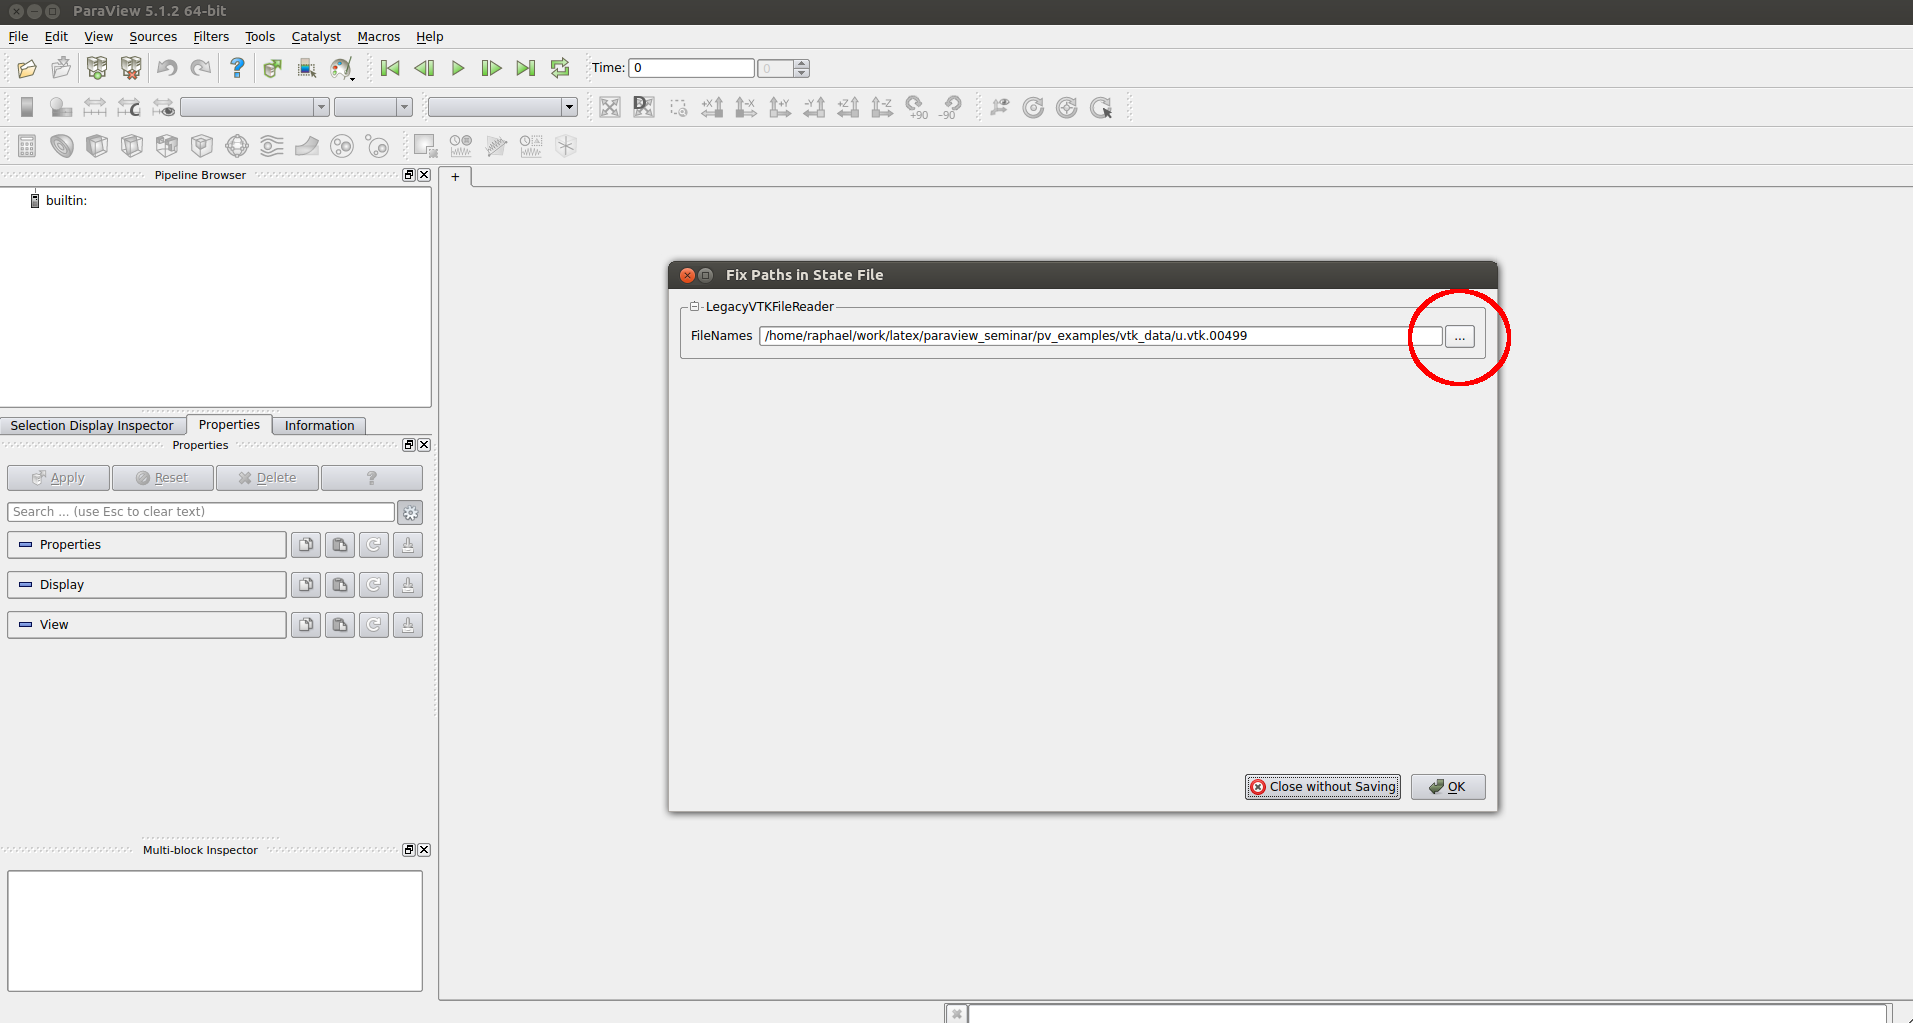
\includegraphics[width=\textwidth]{screenshots/load-state-file.png}
\end{frame}

\begin{frame}
  \frametitle{Examples Files}

    \begin{itemize}
      \item ParaView examples are provided as state files 
      \item Download archive of ParaView examples from:
      \item Extract archive to \kommandozeile{/mypath/to/examples/}
      \kommandozeile{> tar xvfz pv\_examples.tar.gz -C /mypath/to/examples/}
      \item Basic filter examples are located in \kommandozeile{/mypath/to/examples/pv\_examples}
      \item Basic filter examples are located in \kommandozeile{/mypath/to/examples/pv\_examples/BasicFilters}
      \item To load a basic filter example, load the state file and set data path to:
        \kommandozeile{/mypath/to/examples/pv\_examples/vtk\_data/u.vtk}
    \end{itemize}
        

\end{frame}

\begin{frame}
  \frametitle{Basic Filter Gallery I}

    \begin{tikzpicture}%[nodes=draw]

      \node[align=center,scale=0.2,transform shape] (C1) at (0,0)
      {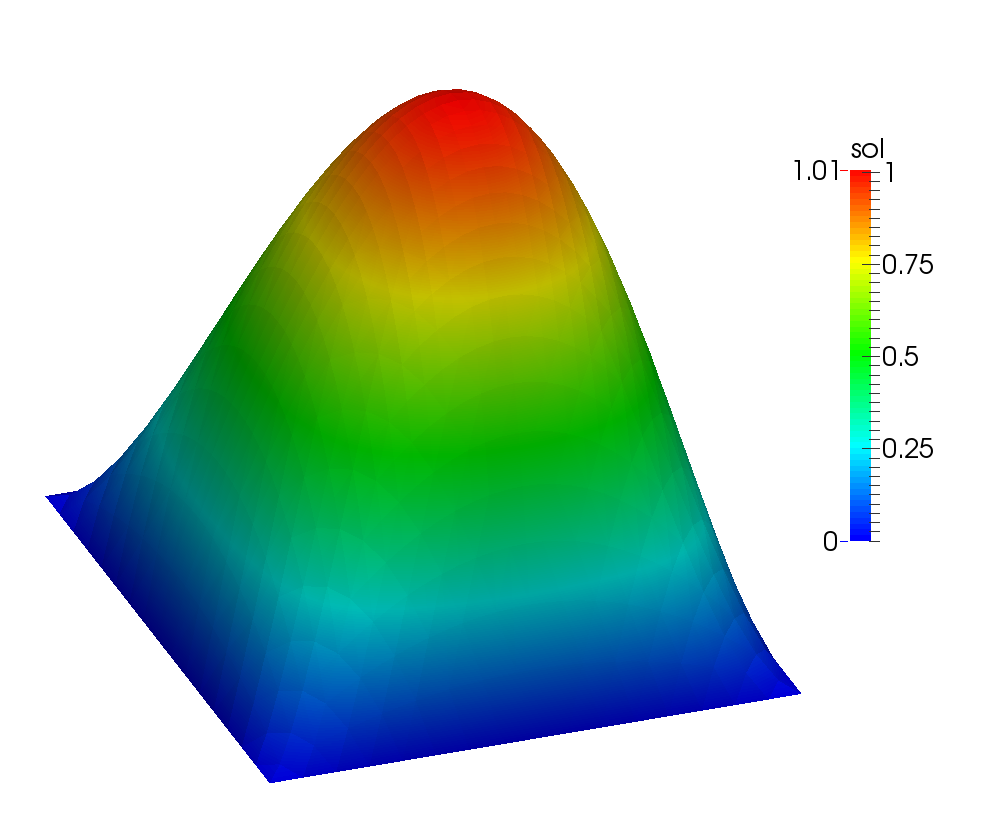
\includegraphics{screenshots/warp-by-scalar.png}};

      \node[align=center,scale=0.2,transform shape] (C2) at (0,-6)
      {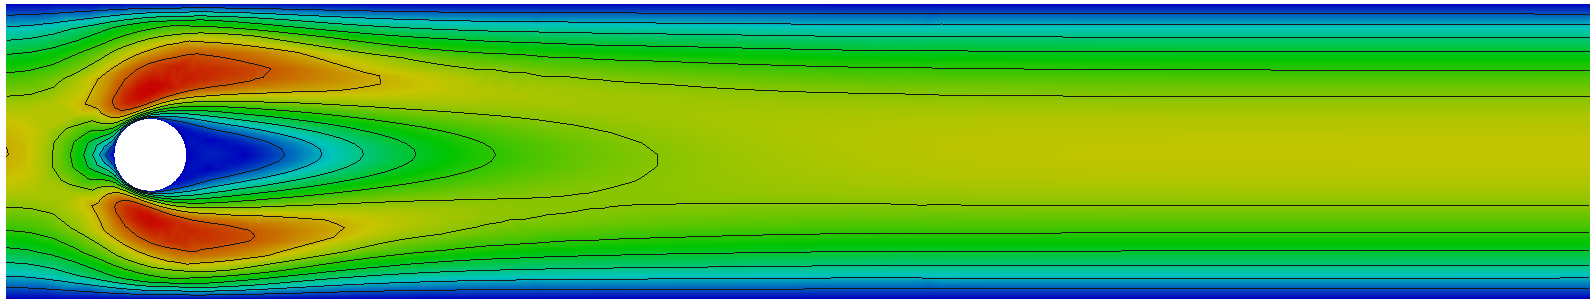
\includegraphics{screenshots/contours.png}};

      \node[align=center,scale=0.2,transform shape] (C3) at (12,-6.05)
      {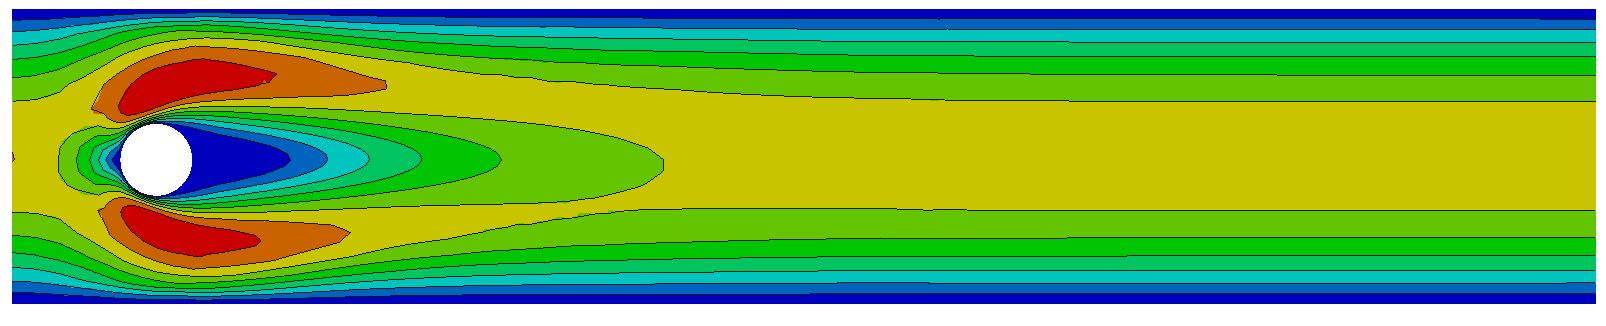
\includegraphics{screenshots/contours_few.png}};

      \node[align=center,scale=0.2,transform shape] (C4) at (12,0)
      {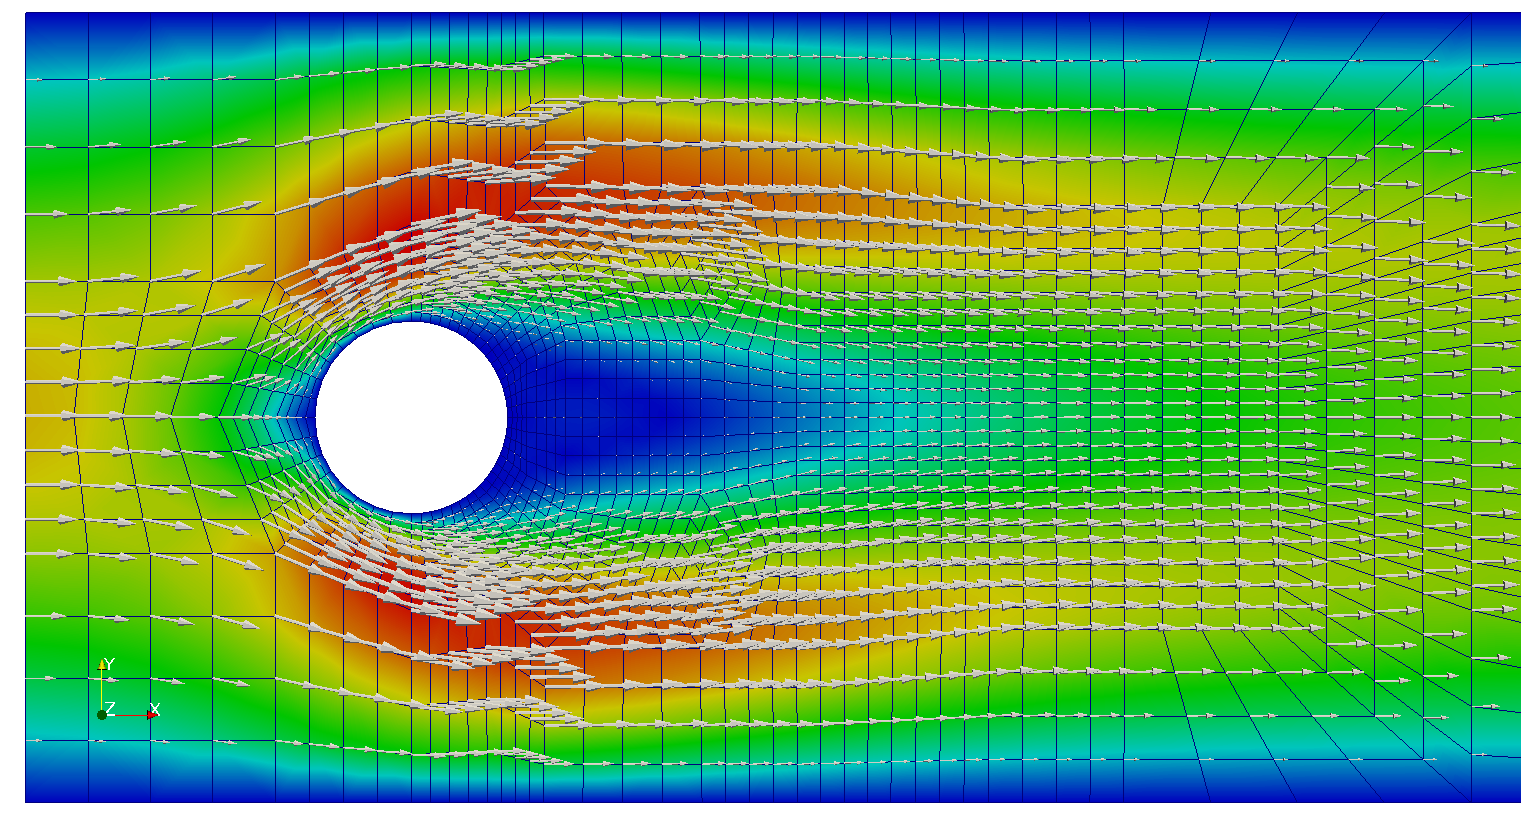
\includegraphics{screenshots/glyphs.png}};

    \end{tikzpicture}

\end{frame}

\begin{frame}

  \frametitle{Basic Filter Gallery II}

    \begin{tikzpicture}%[nodes=draw]

      \node[align=center,scale=0.45,transform shape] (C1) at (0,0)
      {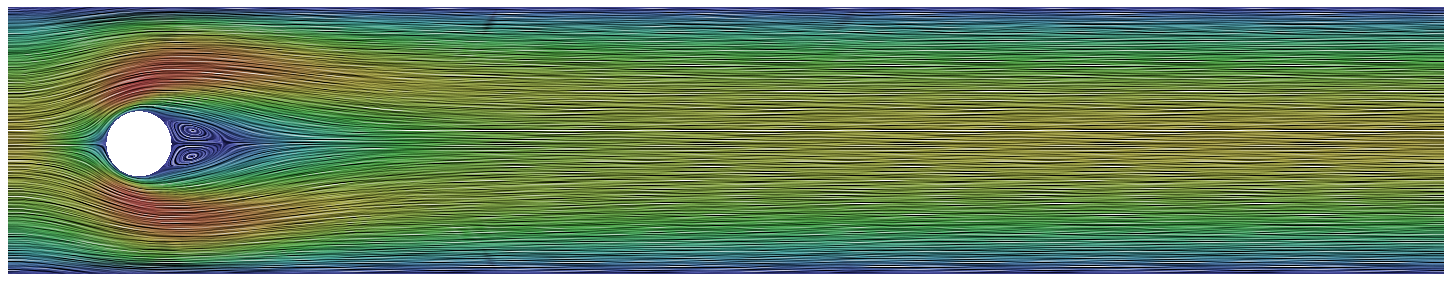
\includegraphics{screenshots/surface_lic_final.png}};

      \node[align=center,scale=0.4,transform shape] (C2) at (0,-6)
      {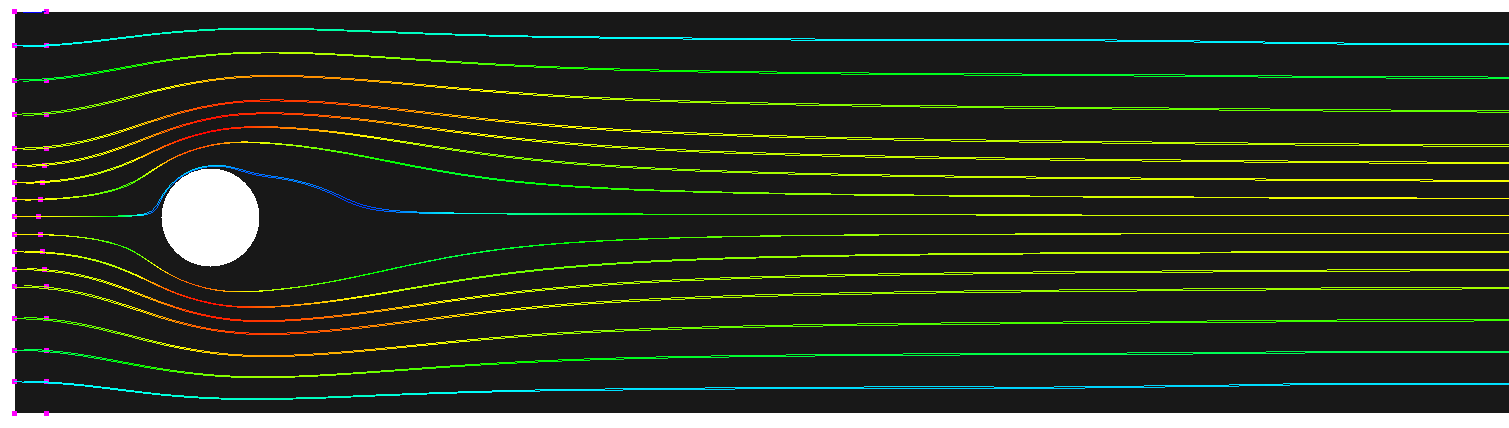
\includegraphics{screenshots/streamlines.png}};


    \end{tikzpicture}

\end{frame}

\begin{frame}

  \frametitle{Configuration of Tracer Filters}

    \begin{itemize}
      \item Tracer type filters need an \keyword{input data set} and a \keyword{seed source}
      \item The input data set is the the flow field  
      \item The seed source is a user-defined starting location for the particles inside the flow field  
    \end{itemize}
    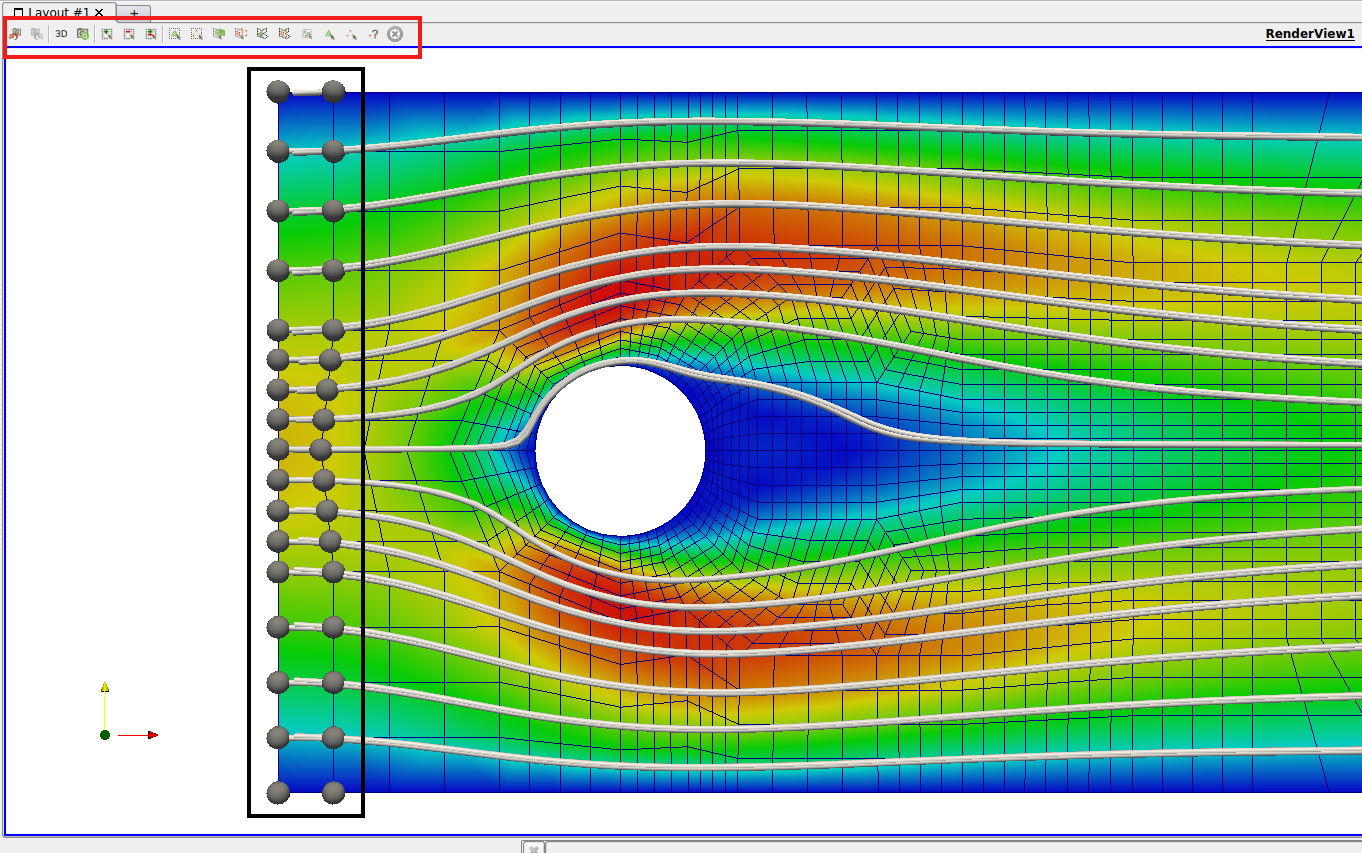
\includegraphics[width=0.5\textwidth]{screenshots/tracer-source.png}

\end{frame}

\begin{frame}

  \frametitle{Advanced Filters: Particle Tracer}

    \begin{itemize}
      \item Used to visualize transient flow data by particles 
      \item A particle path is produced by moving a particle along successive vector fields 
      \item Particle movement can then be animated by the \keyword{Animation Control} 
      \item Particle tracer example location: \kommandozeile{/mypath/to/examples/pv\_examples/AdvancedFilters/particle\_tracer}
    \end{itemize}
    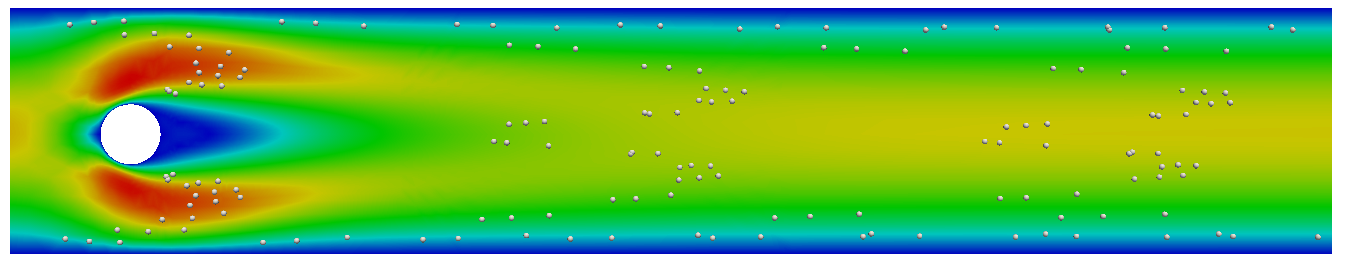
\includegraphics[width=\textwidth]{screenshots/particle-tracer.png}

\end{frame}

\begin{frame}

  \frametitle{List of Useful Filters}

    \begin{itemize}
      \item \keyword{Extract Selection}: Extract a subset from a data set (tracer source, plotting, etc)
      \item \keyword{Extract Surface}: Generates a polygonal surface mesh (exporting, rendering, remeshing) 
      \item \keyword{Clean to Grid}: Removes multiply defined simplices and converts to unstructured mesh
      \item \keyword{Integrate Variables}: Performs numerical integration of the fields defined in the data set on the mesh 
      \item \keyword{Iso-Volume or Iso-Surface}: Constructs a volume or a surface from a function defined on the mesh 
      \item \keyword{Plot Over Line}: Generates a plot of data fields along a line (inflow profiles, etc.) 
      \item \keyword{Calculator}: Use a set of mathematical operations to compute a new data field from existing ones (often used together with integrate variables filter)
    \end{itemize}

\end{frame}

\begin{frame}

  \frametitle{Input Data Formats}

    \begin{itemize}

      \item VTK data formats support polygonal data sets and structured or unstructured meshes 

      \item \keyword{VTK Legacy format .vtk} is a simple format useable for unstructured meshes (not suited for distributed data)  

      \item \keyword{VTK unstructured .vtu} is an xml based format for unstructured meshes   
    \begin{itemize}

      \item Can have the mesh data part encoded in a binary format   

      \item A \keyword{.pvtu} file can be used to reference the partial solutions of a distributed computation   

      \item A \keyword{.pvd} file can be used to add time information   

    \end{itemize}

    \item For further information on VTK file formats see:
      \url{http://www.vtk.org/VTK/img/file-formats.pdf}

  \end{itemize}

\end{frame}

\begin{frame}

  \frametitle{Scripted Postprocessing in ParaView}

  \begin{itemize}

    \item Python interface to access ParaView functionality by scripts

    \item Can be done interactively via a python shell: \keyword{Tools->Python Shell} 

    \item In a 'batch' style by passing a script to the executables \keyword{pvpython} or \keyword{pvbatch} 

    \item Documentation of the ParaView Python interface is under construction at:
      \url{https://www.paraview.org/ParaView3/Doc/Nightly/www/py-doc/}

    \item A trace mechanism is available to generate a PvPython script from a sequence of actions

    \item Beginners should use the trace mechanism (\keyword{Tools->Start Trace}) with the settings \keywords{Show Incremental Trace} and \keywords{only user-modified properties} 

    \item Upon \keyword{Tools->Stop Trace} a file is generated showing the PvPython script equivalent of the user's GUI actions
  \end{itemize}

\end{frame}

\begin{frame}

  \frametitle{PvPython Simple Example}

  \begin{itemize}
      \item PvPython simple example location: \kommandozeile{/mypath/to/examples/pv\_examples/PvPython/paraview\_python}

      \item Navigate to the folder and execute the PvPython script by: \kommandozeile{pvbatch ./python\_test.py \$(pwd)} or for versions higher than 5.1
        \kommandozeile{pvbatch {-}{-}use-offscreen-rendering ./python\_test.py \$(pwd)}

      \item The script will write an image \keyword{res.png} to the directory where you executed it 
      \item \keyword{Exercise:} Try to recreate the python script using the trace mechanism, compare the output images if they are the same.

      \item \keyword{Hint:} Prefer \keyword{pvbatch} over \keyword{pvpython} as pvpython tries to open an X windows which may fail on some computers    
  \end{itemize}

\end{frame}

\begin{frame}

  \frametitle{When to use PvPython}

  \begin{itemize}

    \item Repeated application of filters to a lot of different data sets (parameterize script w.r.t. data set) 

    \item Repeated application of operations that cannot be parametrized by ParaView GUI

    \item Perform an operation that cannot easily be done by ParaView filters 

    \item Quickly and repeatedly generate an ouput of a running simulation 

    \item Generate outputs on remote clusters 

    \item \keyword{ParaView Programmable Filter} or \keyword{Python Calculator} may serve as an alternative 

  \end{itemize}

\end{frame}

\begin{frame}

  \frametitle{Plotting with ParaView}

  \begin{itemize}

      \item PV plotting example: \kommandozeile{/mypath/to/examples/pv\_examples/Plotting/plotting.pvsm}

      \item Common ParaView plotting filters:
      \begin{itemize}

        \item \keyword{Plot Data} 

        \item \keyword{Plot Over Line} 

        \item \keyword{Plot Selection Over Time} 

      \end{itemize}

    \item Data can be exported to .csv to use in your favorite plot generator \keyword{File->Save Data}

    \item ParaView will by default export ALL data fields to the .csv file (even those that you do not want or need for the plot) 

    \item \keyword{Solution 1:} use <awk> to select the data columns you want: \kommandozeile{awk -F \textquotesingle,\textquotesingle $\;$  \textquotesingle\{print \$1 " " \$4\}\textquotesingle} (extract first and fourth column)

    \item \keyword{Solution 2:} Remove unneccessary fields before export: \kommandozeile{/mypath/to/examples/pv\_examples/Plotting/plotting2.pvsm}

  \end{itemize}

\end{frame}

\begin{frame}
  \frametitle{Client-Server Mode}

    \begin{itemize}
      \item In default mode ParaView is both the client and the server
      \item When client/server are different rendering and data processing can
        be handled by different computers 
      \item Simple X forwarding works adequately only if the network speed is fast
      \item Client-Server is preferable to access data on remote (non-local) clusters 
      \item Client-Server steps: \keyword{port forwarding}, \keyword{starting the remote server}, \keyword{connecting the client to the server}  
    \end{itemize}

    \begin{block}{Port Forwarding}
        \begin{itemize}
          \item Establish an ssh tunnel to forward the local port to the remote server: \\  
          \kommandozeile{> ssh lidong1.itmc.tu-dortmund.de \textbackslash}
          \kommandozeile{-L 11111:lidong1.itmc.tu-dortmund.de:11111}
        \end{itemize}
    \end{block}

\end{frame}

\begin{frame}
  %\frametitle{Client-Server Mode II}

    \begin{block}{Start the remote Server}
        \begin{itemize}
          \item Start a ParaView data server on the remote machine  
            \kommandozeile{> pvserver {-}{-}server-port=11111 {-}{-}use-offscreen-rendering}
        \end{itemize}
    \end{block}

    \begin{block}{Connect to the remote Server}
        \begin{itemize}
          \item Start a ParaView client locally  
          \item Press the <Connect> button on the toolbar  
          \item Manually configure the Server dialog:
          \begin{itemize}
            \item Name: myname   
            \item Server Type: Client/Server  
            \item Host: localhost 
            \item Port: 11111 
          \end{itemize}
        \end{itemize}
    \end{block}
  Pitfalls:
    \begin{itemize}
      \item You \textbf{have to} make use the same ParaView version of the client and the server
      \item Check that the port is not occupied, otherwise use a different port: 
      \kommandozeile{> lsof -i:11111}
    \end{itemize}

\end{frame}

\begin{frame}

  \frametitle{Additional ParaView Resources}

  \begin{itemize}
      \item ParaView documentation:\\
        \url{https://www.paraview.org/documentation/}
      \item ParaView Wiki:\\
        \url{https://www.paraview.org/Wiki/ParaView}
      \item ParaView Tutorial:\\
        \url{https://www.paraview.org/Wiki/The\_ParaView\_Tutorial}
      \item ParaView Mailing List:\\
        \url{https://public.kitware.com/mailman/listinfo/paraview}
      \item ParaView Catalyst:\\
        \url{https://www.paraview.org/Wiki/ParaView/Catalyst/Overview}
      \item ParaView Web JavaScript:\\
        \url{www.paraview.org/Wiki/ParaViewWeb\_JavaScript\_Introduction}
  \end{itemize}

\end{frame}


%\begin{frame}
%	\begin{block}{\huge Aufgabe 1 (Hello World)}
%		% <-- Kommentarzeichen

\documentclass{article}

% Praeamble

\begin{document}
    Hello World!
\end{document}

%	\end{block}
%\end{frame}
%\begin{frame}
	\frametitle{Spezielle Zeichen}
	\begin{itemize}
		\item bei Verwendung des ASCII-Zeichensatzes: Buchstaben ohne Umlaute, Zahlen und einige Sonderzeichen
		\item manche Zeichen sind \LaTeX-Steuerzeichen und daher reserviert (\$, \_, \{, \},\textbackslash )
        \item solche Sonderzeichen können durch \textbackslash{} maskiert werden: \\[0.5cm]
		\begin{center}
			\begin{tabular}{|cc|cc|} \hline
				\$ & \textbackslash\$ & \% & \textbackslash\% \\
				\{ & \textbackslash\{ & \} & \textbackslash\} \\
				\# & \textbackslash\# & \_ & \textbackslash\_ \\
				\& & \textbackslash\& & & \\ \hline
			\end{tabular}
		\end{center}
	\end{itemize}
\end{frame}

\begin{frame}[fragile]
	\frametitle{Deutsche Texte - Sprachpakete}
    Ohne weitere Angaben nimmt \LaTeX{} an, dass der eingegebene Text in englischer Sprache ist. Daher muss ggf. ein zusätzliches Sprachpaket eingebunden werden:
	\begin{center}
		\begin{block}{Beispiel-Header: deutsches Sprachpaket}
			\begin{lstlisting}
\documentclass[a4paper]{article}      % DIN-A4 Papierformat
\usepackage[ngerman]{babel}           % deutsche Benennung
\usepackage[utf8]{inputenc}
\begin{document}
  ...
\end{document}
			\end{lstlisting}
		\end{block}
	\end{center} \vspace{-1cm}
	\begin{itemize}
		\item \keyword{babel} sorgt für Unterstützung anderer Sprachen (Formate, Umlaute, Benennungen, Silbentrennung)
		\item \keyword{inputenc} unterstützt die direkte Eingabe von Zeichen über die Tastatur
	\end{itemize}
\end{frame}


\begin{frame}[fragile]
	\frametitle{Deutsche Texte -- Umlaute und Anführungszeichen}
	
	Eingabe deutscher Texte:
	\begin{itemize}
		\item Umlaute: \befehl{"a}, \befehl{"o}, \befehl{"u}, \befehl{ss} für ä, ö, ü, ß
		\item Anführungszeichen: \befehl{glq}, \befehl{grq} bzw. \befehl{glqq}, \befehl{grqq} für \glq einfache\grq~ bzw. \glqq doppelte\grqq~ Anführungszeichen
	\end{itemize}
	\vfill
	
	\latexBeispielDirekt{Beispiel: deutsche Umlaute}{examples/Deutsche_Umlaute/Deutsche_Umlaute}
	\vfill
\end{frame}

\begin{frame}[fragile]
	\frametitle{Deutsche Texte - Silbentrennung}
	\begin{itemize}
		\item erfolgt automatisch
		\item mögliche Trennstellen können  durch \befehl{-} auch angegeben werden, z. B.\\
		\lstinline$Donau\-dampf\-schiff\-fahrts\-gesell\-schaft$\\
		oder für das gesamte Dokument in der Präambel:
		\lstinline$\hypenation{Donau\-dampf\-schiff\-fahrts\-gesell\-schaft}$
	\end{itemize}

\end{frame}

%
%\begin{frame}[fragile]
	\frametitle{Textformatierung -- Schriftstil}
	
	\begin{center}
		\begin{tabular}{l|ll|l}
			Familie & \multicolumn{2}{c|}{Befehle} & Beispiel \\ \hline
			normal (mit Serifen) & \befehl{rmfamily} & \befehl{textr} & \textrm{normal} \\
			serifenfrei & \befehl{sffamily} & \befehl{textsf} & \textsf{serifenfrei} \\
			Schreibmaschine & \befehl{ttfamily} & \befehl{texttt} & \texttt{Schreibmaschine} \\
		\multicolumn{4}{c}{~} \\
			Varianten & \multicolumn{2}{c|}{Befehle} & Beispiel \\ \hline
			aufrecht & \befehl{upshape} & \befehl{textup} & \textup{aufrecht} \\
			italic & \befehl{itshape} & \befehl{textit} & \textit{italic}\\
			Kapitälchen & \befehl{scshape} & \befehl{textsc} & \textsc{Kapitälchen}\\
			fett & \befehl{bfseries} & \befehl{textbf} & \textbf{fett}\\
			unterstrichen & ~ & \befehl{underline} & \underline{unterstrichen}
		\end{tabular}
	\end{center}
\end{frame}

\begin{frame}[fragile]
	\frametitle{Textformatierung -- Schriftgröße}
	\begin{center}
		\begin{tabular}{ll}
		\befehl{tiny} & \tiny{winzig} \\
		\befehl{small} & \small{klein} \\
		\befehl{footnotesize} & {\fontsize{14}{14}\selectfont{}Fußnotengröße}\\
		\befehl{normalsize} & normale Größe\\
		\befehl{large} & {\fontsize{25}{25}\selectfont{}groß} \\
		\befehl{Large} & {\fontsize{30}{30}\selectfont{}größer} \\
		\befehl{huge} & {\fontsize{40}{40}\selectfont{}riesig} \\
		\befehl{Huge} & {\fontsize{50}{50}\selectfont{}Riesig}
		\end{tabular}
	\end{center}
	\vfill
	\begin{itemize}
		\item für einige Wörter: \lstinline${\huge riesig}$
		\item für ganze Absätze: \lstinline$\begin{tiny} ... \end{tiny}$
		\item alternativ: punktgenau durch \lstinline${\fontsize{40}{48}\selectfont{}Test}$\\
		das erste Argument gibt die Schriftgröße an, das zweite den Grundlinienabstand
	\end{itemize}
\end{frame}



%\begin{frame}[fragile]
	\frametitle{Textformatierung -- minipages}
	\begin{itemize}
		\item die \keyword{minipage}-Umgebung wird genutzt, wenn in Boxen komplexere Inhalte  dargestellt werden sollen
		\item es muss die Breite angegeben werden
	\end{itemize}
	\latexBeispielDirekt{Beispiel: minipages}{examples/minipages/minipages.tex}
\end{frame}

\begin{frame}[fragile]
	\frametitle{Textformatierung -- Absatzausrichtung} \vspace{-0.7cm}
	\latexBeispielDirekt{Beispiel: Absatzausrichtung}{examples/absatzausrichtung/absatzausrichtung.tex}
	\vfill
\begin{itemize}
	\item Standard: Blocksatz
	\item alternativ kann man auch die Befehle \befehl{raggedleft}, \befehl{raggedright} und \befehl{centering} verwenden (statt den obigen Umgebungen)
\end{itemize}
\end{frame}

\begin{frame}[fragile]
	\frametitle{Textformatierung - Zitate und Gedichte}
	\latexBeispielDirektKlein{Beispiel: Zitate und Gedichte}{examples/Zitate_und_Gedichte/Zitate_und_Gedichte.tex}
\end{frame}

\begin{frame}[fragile]
	\frametitle{Text ohne Formatierung}
	\begin{itemize}
		\item um Programmcode oder Beispiele ohne Formatierung auszugeben, gibt es die \keyword{verbatim}-Umgebung
		\item innerhalb eines Textes kann man den Befehl \befehl{verb} nutzen; das erste Zeichen nach dem Befehl wird dann als Endmarker interpretiert
	\end{itemize}\vfill
	\latexBeispielDirekt{Beispiel: \keyword{verbatim}-Umgebung}{examples/verbatim/verbatim.tex}
\end{frame}

\begin{frame}[fragile]
	\frametitle{Randnotizen und Fußnoten}
	\latexBeispielDatei{Beispiel: Randnotiz und Fußnote}{examples/Randnotiz_und_Fussnote/Randnotiz_und_Fussnote}
\end{frame}
%%\begin{frame}[fragile]
	\frametitle{Dokumentenklasse}
	
	\begin{block}{Allgemeine Form}
		\lstinline$\documentclass[option1,option2]{klasse}$
	\end{block}
	\vfill
	einige verfügbare Klassen:
	\begin{itemize}
		\item \emphkeyword{article}, \emphkeyword{scrartcl} für Artikel, Ausarbeitungen oder Berichte
		\item \emphkeyword{report}, \emphkeyword{scrreprt} für Ausarbeitungen, Diplomarbeiten, Skripten oder Dissertationen
		\item \emphkeyword{book}, \emphkeyword{scrbook} für Bücher
		\item \emphkeyword{letter}, \emphkeyword{scrlttr2} für Briefe
	\end{itemize}
	\vfill
\end{frame}


\begin{frame}[fragile]
	\frametitle{Dokumentenklasse -- häufig benutzte Optionen}
	
	\begin{tabular}{rl}
		\emphkeyword{draft} & Entwurfsmodus (markiert überstehenden Text, zeigt Grafiken als Box) \\
		\emphkeyword{11pt} & Schriftgr\"o\ss{}e 11 Punkte \\
		\emphkeyword{12pt} & Schriftgr\"o\ss{}e 12 Punkte\\
		\emphkeyword{a4paper} & Gr\"o\ss{}en anpassen f\"ur Din A4\\
		\emphkeyword{titlepage} & Titelseite erzwingen f\"ur \keyword{\texttt{article}}\\
		\emphkeyword{twocolumn} & zweispaltiges Dokument\\
		\emphkeyword{twoside} & Vorder- und R\"uckseite der Seiten wird bedruckt\\
		\emphkeyword{fleqn} & Formeln linksb\"undig setzen\\
		\emphkeyword{leqno} & Nummerierung von Formeln links statt rechts
	\end{tabular}
\end{frame}


\begin{frame}
	\frametitle{Titelseite aus Metadaten}
	
	\only<1>{
	\latexBeispielDateiCodeAnmerkungen{automatisch generierte Titelseite}{examples/Titelseite/Titelseite}{
	\begin{tabular}{rp{6cm}}
		\keyword{\~} & unzerbrechliches Leer\-zeichen\\
		\befehl{title} & Titel des Dokuments \\
		\befehl{author} & Autoren (Schlüsselwort \befehl{and} bei Angabe mehrerer Autoren) \\
		\befehl{date} & Veröffentlichungsdatum\\
		\befehl{maketitle} & generiert die Titelseite aus den Metadaten
	\end{tabular}
	}}
	\only<2>{\latexBeispielDatei{automatisch generierte Titelseite}{examples/Titelseite/Titelseite}}
\end{frame}

\begin{frame}
	\frametitle{Eigene Titelseiten}
	\begin{itemize}
		\item um die Titelseite selbst zu gestalten, kann man die \emphkeyword{titlepage}-Umgebung nutzen
	\end{itemize} \vfill
		\latexBeispielDirektFake{Beispiel: eigene Titelseite}{examples/Eigene_Titelseite/Eigene_Titelseite}{\textbf{\Huge Nicht wichtig}\\geschrieben von mir\ldots} \vfill
	\begin{itemize}
		\item die Titelseite taucht an der Stelle im Text auf, an der sie definiert wird
		\item bei einigen Dokumentenklassen (z. B. \emphword{book}) nimmt die Titelseite auch eine ganze Seite ein
	\end{itemize}
\end{frame}

\begin{frame}[fragile]
	\frametitle{Abstract (Zusammenfassung)}
	\begin{itemize}
		\item durch die \emphkeyword{abstract}-Umgebung kann man eine Zusammenfassung des Inhalts angeben
	\end{itemize} \vfill
	\latexBeispielDirektFake{Beispiel: Abstract (Zusammenfassung)}{examples/abstract/abstract}{
	\begin{center} \textbf{\LARGE Abstract} \end{center} \noindent \ldots Zusammenfassung des Textes \ldots} \vfill
	\begin{itemize}
        \item der angezeigte Name \glqq Abstract\grqq{} kann individualisiert werden:\\
		\lstinline$\renewcommand{\abstractname}{MeinName}$
	\end{itemize}
\end{frame}

\begin{frame}
	\frametitle{Strukturierung des Dokuments}
	
	\begin{itemize}
		\item Gliederung in Kaptiel und Unterkapitel
		\begin{itemize}
			\item \befehl{part\{\}} (nicht in allen Dokumentklassen)
			\item \befehl{chapter\{\}} (nicht in allen Dokumentklassen)
			\item \befehl{section\{\}}
			\item \befehl{subsection\{\}}
			\item \befehl{subsubsection\{\}}
			\item \befehl{paragraph\{\}}
			\item \befehl{subparagraph\{\}}
		\end{itemize}
		\item in den geschweiften Klammern \{\} kann der Name des jeweiligen (Unter-)Kapitels angegeben werden
		\item mit dem Befehl \befehl{appendix} kann markiert werden, dass die nachfolgenden (Unter-)Kapitel zum Anhang gehören
	\end{itemize}
\end{frame}

\begin{frame}[fragile]
	\frametitle{Mehrere Quelldateien}
	\begin{itemize}
		\item um Quelltext aus einer anderen Datei einzufügen, wird der \befehl{input}-Befehl genutzt\\
		\lstinline$\input{datei}$
		\item um ganze Kapitel einzubinden, verwendet man stattdessen den Befehl\\
		\lstinline$\include{kapitel}$
		\item zur Gliederung des \LaTeX-Quellcodes schreibt man Kapitel in jeweils eigene Dateien\\
		\lstinline$\include{kapitel1}$\\
		\lstinline$\include{kapitel2}$\\
		usw.
	\end{itemize}
\end{frame}

%\begin{frame}
%	\vspace{-1cm}
%	\begin{block}{\huge Aufgabe 2 (Ein erstes Dokument)}
%		\input{../exercises/exercises/ein_erstes_eigenes_dokument}
%	\end{block}
%	\vfill
%	\begin{block}{\huge Aufgabe 3 (Umlaute)}
%		\input{../exercises/exercises/umlaute}
%	\end{block}
%\end{frame}
%\begin{frame}
%	\begin{block}{\huge Aufgabe 4 (Zusammensetzen des Dokuments aus mehreren Dateien)}
%		\input{../exercises/exercises/zusammensetzen}
%	\end{block}
%\end{frame}
%\begin{frame}[fragile]
	\frametitle{Aufzählungen}
	\vspace{-0.5cm}
	drei Grundarten von Aufzählungen: \\
	\begin{tabular}{rl}
		\emphkeyword{itemize} & einfache Aufzählung\\
		\emphkeyword{enumerate} & nummerierte Aufzählung\\
		\emphkeyword{description} & Beschreibung
	\end{tabular}\par \vfill
	
	\begin{columns}[T]
		\begin{column}{0.31\textwidth}
			\begin{block}{\tt\bfseries itemize}
				\begin{itemize}
					\item A \item B \item C
				\end{itemize} 
				\begin{lstlisting}
\begin{itemize}
  \item A
  \item B
  \item C
\end{itemize}
				\end{lstlisting}
			\end{block}
		\end{column}
		\begin{column}{0.31\textwidth}
			\begin{block}{\tt\bfseries enumerate}
				\begin{enumerate}
					\item A \item B \item C
				\end{enumerate} 
				\begin{lstlisting}
\begin{enumerate}
  \item A
  \item B
  \item C
\end{enumerate}
				\end{lstlisting}
			\end{block}
		\end{column}
		\begin{column}{0.31\textwidth}
			\begin{block}{\tt\bfseries description}
				\begin{description}
					\item[A] \ldots \item[B] \ldots \item[C] \ldots
				\end{description} 
				\begin{lstlisting}
\begin{description}
  \item[A] \ldots
  \item[B] \ldots
  \item[C] \ldots
\end{description}
				\end{lstlisting}
			\end{block}
		\end{column}
	\end{columns}
\end{frame}

\begin{frame}[fragile]
	\frametitle{Verschachtelte Aufzählungen}
	\vspace{-0.9cm}
	\latexBeispielDirekt{Beispiel: verschachtelte Aufzählung}{examples/Verschachtelte_Aufzaehlung/Verschachtelte_Aufzaehlung}
\end{frame}
%\begin{frame}
%	\begin{block}{\huge Aufgabe 5 (Listen und Aufzählungen)}
%		\input{../exercises/exercises/listen_und_aufzaehlungen}
%	\end{block}
%\end{frame}
%\begin{frame}[fragile]
	\frametitle{Tabellen - ein einfaches Beispiel}
	\vspace{-0.9cm}
	\latexBeispielDirekt{Beispiel: einfache Tabelle}{examples/Tabelle_einfach/Tabelle_einfach}
	\vfill
	Tabellenformatierung:\\[0.2cm]
	\begin{tabular}{rlcrl}
		\emphkeyword{l} & linksbündig ausrichten &~~~~~~ & \emphkeyword{|} & einfacher vertikaler Trennstrich \\
		\emphkeyword{c} & zentriert ausrichten && \emphkeyword{||} & doppelter vertikaler Trennstrich\\
		\emphkeyword{r} & rechtsbündig ausrichten && \emphkeyword{@\{text\}} & benutzerdefiniertes Trennzeichen \\
		\emphkeyword{p\{n\}} & Spalte mit fester Breite \keyword{n}
	\end{tabular}
\end{frame}

\begin{frame}
	\frametitle{Tabellen - mehrspaltige Zellen}
	\vspace{-0.9cm}
	\latexBeispielDirekt{Beispiel: mehrspaltige Zellen}{examples/Tabelle_multicolumn/Tabelle_multicolumn}
	\vfill
	Tabellenformatierung:\\[0.2cm]
	\begin{tabular}{rl}
		\emphkeyword{\textbackslash{}hline} & horizontale Linie über die ganze Breite \\
		\emphkeyword{\textbackslash{}vline} & vertikaler Line innerhalb einer Zeile \\
		\emphkeyword{\textbackslash{}cline\{m-n\}} & horizontale Linie von Spalte \keyword{m} bis Spalte \keyword{n}\\
		\emphkeyword{\textbackslash{}multicolumn\{n\}\{format\}\{Inhalt\}} & Zelle über \keyword{n} Spalten
	\end{tabular}
\end{frame}
%\begin{frame}
%	\begin{block}{\huge Aufgabe 6 (Tabellen)}
%		\begin{frame}[fragile]
	\frametitle{Tabellen - ein einfaches Beispiel}
	\vspace{-0.9cm}
	\latexBeispielDirekt{Beispiel: einfache Tabelle}{examples/Tabelle_einfach/Tabelle_einfach}
	\vfill
	Tabellenformatierung:\\[0.2cm]
	\begin{tabular}{rlcrl}
		\emphkeyword{l} & linksbündig ausrichten &~~~~~~ & \emphkeyword{|} & einfacher vertikaler Trennstrich \\
		\emphkeyword{c} & zentriert ausrichten && \emphkeyword{||} & doppelter vertikaler Trennstrich\\
		\emphkeyword{r} & rechtsbündig ausrichten && \emphkeyword{@\{text\}} & benutzerdefiniertes Trennzeichen \\
		\emphkeyword{p\{n\}} & Spalte mit fester Breite \keyword{n}
	\end{tabular}
\end{frame}

\begin{frame}
	\frametitle{Tabellen - mehrspaltige Zellen}
	\vspace{-0.9cm}
	\latexBeispielDirekt{Beispiel: mehrspaltige Zellen}{examples/Tabelle_multicolumn/Tabelle_multicolumn}
	\vfill
	Tabellenformatierung:\\[0.2cm]
	\begin{tabular}{rl}
		\emphkeyword{\textbackslash{}hline} & horizontale Linie über die ganze Breite \\
		\emphkeyword{\textbackslash{}vline} & vertikaler Line innerhalb einer Zeile \\
		\emphkeyword{\textbackslash{}cline\{m-n\}} & horizontale Linie von Spalte \keyword{m} bis Spalte \keyword{n}\\
		\emphkeyword{\textbackslash{}multicolumn\{n\}\{format\}\{Inhalt\}} & Zelle über \keyword{n} Spalten
	\end{tabular}
\end{frame}
%	\end{block}
%\end{frame}
%
\begin{frame}[fragile]
	\frametitle{Mathematik -- Formeln im Fließtext}
	\begin{itemize}
        \item Formeln müssen in \LaTeX{} markiert werden, damit sie korrekt interpretiert werden
		\item im Mathematik-Modus werden Leerzeichen ignoriert und Buchstabenketten als einzelne Zeichen betrachtet
	\end{itemize}
	\vfill
	\latexBeispielDirekt{Beispiel: Formeln im Fließtext}{examples/Formeln_im_Fliesstext/Formeln_im_Fliesstext}
\end{frame}

\begin{frame}[fragile]
	\frametitle{Mathematik -- Formeln in eigenem Absatz}
	\begin{itemize}
		\item soll eine Formel abgesetzt dargestellt werden, so benutzt man die \keyword{displaymath}-Umgebung oder die Kurzschreibweise \lstinline$\[...\]$
	\end{itemize}
	\vfill
	\latexBeispielDirekt{Beispiel: Formeln in eigenem Absatz}{examples/Formeln_eigener_Absatz/Formeln_eigener_Absatz}
\end{frame}

\begin{frame}[fragile]
	\frametitle{Mathematik -- nummerierte Gleichungen}
	\begin{itemize}
		\item Gleichungen können mit der \keyword{equation}-Umgebung automatisch fortlaufend nummeriert werden
		\item mittels der \keyword{align}-Umgebung können mehrzeilige Formeln nummeriert und ausgerichtet werden
		\item \befehl{nonumber} unterdrückt in der \keyword{align}-Umgebung die Nummerierung einer Zeile
	\end{itemize}
	\vfill
	\latexBeispielDirektKlein{Beispiel: mehrzeilige Gleichungen}{examples/Formeln_mehrzeilig/Formeln_mehrzeilig}
\end{frame}


%\begin{frame}[fragile]
	\frametitle{Mathematik -- Unterschiede bei der Darstellung}
	\begin{itemize}
		\item Formeln werden innerhalb der \keyword{math}-Umgebung anders dargestellt als in der \keyword{displaymath}-Umgebung
	\end{itemize}
	\begin{center}
		\begin{tabular}{c|c|c}
			\LaTeX-Befehl & \keyword{math} & \keyword{displaymath} \\ \hline
			\lstinline$\lim_{x \ra \infty} \ra 0$
			&
			\begin{math}
				\lim_{x \to \infty} \ra 0
			\end{math}
			&\begin{minipage}{4cm}
				\begin{displaymath}
					\lim_{x \ra \infty} \ra 0
				\end{displaymath}
			\end{minipage}
		\end{tabular}
	\end{center}
	\begin{itemize}
		\item mit dem Befehl \befehl{displaystyle} bzw. \befehl{textstyle} kann das jeweils andere Verhalten erzwungen werden
	\end{itemize}
	\latexBeispielDirekt{Beispiel: \keyword{textstyle} und \keyword{displaystyle}}{examples/Formeln_Darstellung/Formeln_Darstellung}
\end{frame}

\begin{frame}
	\frametitle{Mathematik -- Symbole}
	
	\emphword{Logik}
	\begin{center}
		\begin{tabular}{ll|ll|ll|ll|ll}
			\befehl{exists} & $\exists$ & \befehl{forall} & $\forall$ & \befehl{neg} & $\neq$ & \befehl{in} & $\in$ & \befehl{emptyset} & $\emptyset$ \\
			\befehl{notin} & $\notin$ & \befehl{ni} & $\ni$ & \befehl{land} & $\land$ & \befehl{lor} & $\lor$ & \befehl{varnothing} & $\varnothing$\\
			\befehl{setminus} & $\setminus$ & \befehl{implies} & $\implies$ & \befehl{iff} & $\iff$ & \befehl{to} & $\to$ & \befehl{top} & $\top$
		\end{tabular}
	\end{center}\vspace{1cm}
	
	\emphword{Pfeile} \vspace{-0.9cm}
	\begin{center}
		\begin{tabular}{ll|ll|ll|ll}
			\befehl{leftarrow} & $\la$ & \befehl{rightarrow} & $\ra$ & \befehl{uparrow} & $\uparrow$ & \befehl{downarrow} & $\downarrow$ \\
			\befehl{Leftarrow} & $\La$ & \befehl{Rightarrow} & $\Ra$ & \befehl{Uparrow} & $\Uparrow$ & \befehl{Downarrow} & $\Downarrow$ \\
			\befehl{leftrightarrow} & $\leftrightarrow$ & \befehl{Leftrightarrow} & $\Leftrightarrow$ & \befehl{nearrow} & $\nearrow$ & \befehl{searrow} & $\searrow$ \\
			 \befehl{updownarrow} & $\updownarrow$ & \befehl{Updownarrow} & $\Updownarrow$ & \befehl{swarrow} & $\swarrow$ & \befehl{nwarrow} & $\nwarrow$ \\
			 \befehl{longleftarrow} & $\longleftarrow$ & \befehl{Longleftarrow} & $\Longleftarrow$ & \befehl{mapsto} & $\mapsto$ & \befehl{leadsto} & $\leadsto$ \\
			 \befehl{longrightarrow} & $\longrightarrow$ & \befehl{Longrightarrow} & $\Longrightarrow$
		\end{tabular}
	\end{center}
\end{frame}

\begin{frame}
	\frametitle{Mathematik -- Symbole}
	\emphword{Sonstige}
	\begin{center}
		\begin{tabular}{ll|ll|ll|ll|ll}
			\befehl{partial} & $\partial$ & \befehl{nabla} & $\nabla$ & \befehl{infty} & $\infty$ & \befehl{ell} & $\ell$ & \befehl{imath} & $\imath$ \\
			\befehl{jmath} & $\jmath$ & \befehl{Re} & $\Re$ & \befehl{Im} & $\Im$ & \befehl{dots} & $\dots$ & \befehl{cdots} & $\cdots$ \\
			\befehl{vdots} & $\vdots$ & \befehl{ddots} & $\ddots$ & \befehl{ldots} & $\ldots$ & \befehl{pm} & $\pm$ & \befehl{mp} & $\mp$
		\end{tabular}
	\end{center} \vspace{1cm}
	

\end{frame}


\begin{frame}
	\frametitle{Mathematik -- Griechische Buchstaben}
	\vspace{-0.5cm}
	\begin{center}
\begin{tabular}{ll|ll||ll}
\befehl{alpha}      & $\alpha$  & 
\befehl{xi}         & $\xi$ &
\befehl{Gamma}      & $\Gamma$ \\

\befehl{beta}       & $\beta$  & 
\befehl{pi}         & $\pi$ &
\befehl{Delta}      & $\Delta$ \\

\befehl{gamma}      & $\gamma$  & 
\befehl{varpi}      & $\varpi$ &
\befehl{Theta}      & $\Theta$ \\

\befehl{delta}      & $\delta$  & 
\befehl{rho}        & $\rho$ &
\befehl{Lambda}     & $\lambda$ \\

\befehl{epsilon}    & $\epsilon$  & 
\befehl{varrho}     & $\varrho$ &
\befehl{Xi}         & $\Xi$ \\

\befehl{varepsilon} & $\varepsilon$  & 
\befehl{sigma}      & $\sigma$ &
\befehl{Pi}         & $\Pi$ \\

\befehl{zeta}       & $\zeta$  & 
\befehl{varsigma}   & $\varsigma$ &
\befehl{Sigma}      & $\Sigma$ \\

\befehl{eta}        & $\eta$  & 
\befehl{tau}        & $\tau$ &
\befehl{Upsilon}    & $\Upsilon$ \\

\befehl{theta}      & $\theta$  & 
\befehl{upsilon}    & $\upsilon$ &
\befehl{Phi}        & $\Phi$ \\

\befehl{vartheta}   & $\vartheta$  & 
\befehl{phi}        & $\phi$ &
\befehl{Psi}        & $\Psi$ \\

\befehl{iota}       & $\iota$  & 
\befehl{varphi}     & $\varphi$ &
\befehl{Omega}      & $\Omega$ \\

\befehl{kappa}      & $\kappa$  & 
\befehl{chi}        & $\chi$ \\

\befehl{lambda}     & $\lambda$  & 
\befehl{psi}        & $\psi$ &
                & \\

\befehl{mu}         & $\mu$  & 
\befehl{omega}      & $\omega$ &
                & \\

\befehl{nu}         & $\nu$ &
                &       &
                & \\

\end{tabular}
\end{center}
\end{frame}

\begin{frame}
	\frametitle{Mathematik -- binäre Operatoren}
	\begin{center}
\begin{tabular}{ll|ll|ll}
\befehl{leq} & $\leq$ &
\befehl{geq} & $\geq$ &
\befehl{equiv} & $\equiv$
\\
\befehl{models} & $\models$ &
\befehl{prec} & $\prec$ &
\befehl{succ} & $\succ$
\\
\befehl{sim} & $\sim$ &
\befehl{perp} & $\perp$ &
\befehl{preceq} & $\preceq$
\\
\befehl{succeq} & $\succeq$ &
\befehl{simeq} & $\simeq$ &
\befehl{mid} & $\mid$
\\
\befehl{ll} & $\ll$ &
\befehl{gg} & $\gg$ &
\befehl{asymp} & $\asymp$ 
\\
\befehl{parallel} & $\parallel$ &
\befehl{subset} & $\subset$ &
\befehl{supset} & $\supset$
\\
\befehl{approx} & $\approx$ &
\befehl{bowtie} & $\bowtie$ &
\befehl{subseteq} & $\subseteq$
\\
\befehl{supseteq} & $\supseteq$ &
\befehl{cong} & $\cong$ &
\befehl{sqsubset} & $\sqsubset$
\\
\befehl{sqsupset} & $\sqsupset$ &
\befehl{neq} & $\neq$ &
\befehl{smile} & $\smile$
\\
\befehl{sqsubseteq} & $\sqsubseteq$ &
\befehl{sqsupseteq} & $\sqsupseteq$ &
\befehl{doteq} & $\doteq$
\\
\befehl{frown} & $\frown$ &
\befehl{in} & $\in$ &
\befehl{ni} & $\ni$
\\
\befehl{propto} & $\propto$ &
= & $=$ &
\befehl{vdash} & $\vdash$
\\
\befehl{dashv} & $\dashv$ &
< & $<$ &
> & $>$
\end{tabular}
\end{center}
\end{frame}

\begin{frame}
	\frametitle{Mathematik -- Negation von Operatoren}
	\begin{itemize}
		\item oftmals kann ein Operator negiert werden, indem der Befehl \befehl{not} vorgestellt wird
		\begin{center}
			\begin{tabular}{ll|ll|ll}
				\befehl{not<} & $\not<$ & \befehl{not}\befehl{leq} & $\not\leq$ & \befehl{not}\befehl{subseteq} $\not\subseteq$
			\end{tabular}
		\end{center}
		\item einige Operatoren haben dafür jedoch spezielle Symbole
		\begin{center}
			\begin{tabular}{ll|ll}
				\befehl{not=} & $\not=$ & \befehl{neq} & $\neq$ \\
				\befehl{not}\befehl{in} & $\not\in$ & \befehl{notin} & $\notin$
			\end{tabular}
		\end{center}
	\end{itemize}
\end{frame}

\begin{frame}
	\frametitle{Mathematik  -- gestapelte Operatoren}
	\begin{itemize}
		\item manchmal werden Anmerkungen an Relationen geschrieben oder eigene Operatoren definiert
		\item dazu eignet sich der \befehl{stackrel} Befehl
	\end{itemize}
	\vfill
	\latexBeispielDirekt{Beispiel: \befehl{stackrel} Befehl}{examples/Mathematik_stackrel/Mathematik_stackrel}
\end{frame}

\begin{frame}
	\frametitle{Mathematik -- Funktionen}
	\begin{center}
\begin{tabular}{lllll}
\befehl{arccos} \quad &
\befehl{arcsin} \quad &
\befehl{arctan} \quad &
\befehl{arg} \quad &
\befehl{cos} \\[0.5cm]
\befehl{cosh} &
\befehl{cot} &
\befehl{coth} &
\befehl{csc} &
\befehl{deg} \\[0.5cm]
\befehl{det} &
\befehl{dim} &
\befehl{exp} &
\befehl{gcd} &
\befehl{hom} \\[0.5cm]
\befehl{inf} &
\befehl{ker} &
\befehl{lg} &
\befehl{lim} &
\befehl{liminf} \\[0.5cm]
\befehl{limsup} &
\befehl{ln} &
\befehl{log} &
\befehl{max} &
\befehl{min} \\[0.5cm]
\befehl{Pr} &
\befehl{sec} &
\befehl{sin} &
\befehl{sinh} &
\befehl{sup} \\[0.5cm]
\befehl{tan} &
\befehl{tanh} &
\end{tabular}
\end{center}
\end{frame}

\begin{frame}
	\frametitle{Mathematik -- Hoch- und Tiefstellung}
	\begin{itemize}
		\item um Exponenten oder Indizes anzugeben, benutzt man zur Hochstellung das Zeichen \lstinline$^$ und zur Tiefstellung das Zeichen \lstinline$_$
		\item möchte man mehr als ein Zeichen hoch- oder tiefstellen, muss man den Term in geschweiften Klammern angeben
		\item die Reihenfolge ist egal
		\item mit den Befehlen \befehl{limits} und \befehl{nolimits} kann man die Darstellung für das Hoch- bzw. Tiefstellen beinflussen
	\end{itemize}
	\vfill
	\latexBeispielDirekt{Beispiel: Hoch- und Tiefstellung}{examples/Mathematik_HochTief/Mathematik_HochTief}
\end{frame}

\begin{frame}[fragile]
	\frametitle{Mathematik -- Brüche}
	\begin{itemize}
		\item der \befehl{frac} Befehl dient der Darstellung von Brüchen und erfordert zwei Argumente
	\end{itemize}
	\vfill
	\latexBeispielDirekt{Beispiel: Brüche}{examples/Mathematik_frac/Mathematik_frac}
\end{frame}

\begin{frame}[fragile]
	\frametitle{Mathematik -- Wurzel und Binomialkoeffizient}
	\emphword{Wurzel}
	\begin{itemize}
		\item der Wurzelbefehl heißt \befehl{sqrt}
		\item optional kann der Parameter \keyword{n} angeben werden ($n = 2$:  Quadratwurzel)
	\end{itemize}
	\vfill
	\emphword{Binomialkoeffizient}
	\begin{itemize}
		\item zur Darstellung des Binomialkoeffizienten dient der Befehl \befehl{choose}
		\item das erste Argument wird oben, das zweite unten gesetzt
	\end{itemize}
	\vfill
	\latexBeispielDirekt{Beispiel: Wurzeln, Binomialkoeffizienten}{examples/Mathematik_Wurzel_Binom/Mathematik_Wurzel_Binom}
\end{frame}

\begin{frame}[fragile]
	\frametitle{Mathematik -- Klammerung} \vspace{-0.6cm}
	\begin{itemize}
		\item Klammern: \keyword{() [] \{\} ||} \befehl{langle}\befehl{rangle} \befehl{lfloor}\befehl{rfloor} \befehl{lceil}\befehl{rceil}
			\[ (\,) \quad [\,] \quad \{\,\} \quad |\,| \quad \langle \, \rangle \quad \lfloor \, \rfloor \quad \, \lceil \, \rceil \]
		\item die Größe der Klammern kann manuell durch die Befehle \befehl{big}, \befehl{Big}, \befehl{bigg}, \befehl{Bigg} variert werden
			\[ ( \big( \Big( \bigg( \Bigg( \, \Bigg) \bigg) \Big) \big) ) \]
		\item besser: die Klammergröße kann automatisch gesetzt werden
		\item dazu setzt man den einzuklammernden Begriff zwischen die Befehle \befehl{left} und \befehl{right}; direkt darauf folgt das zu verwendende Klammerzeichen\\
		\item möchte man auf einer Seite keine Klammern haben, verwendet man als Klammerzeichen \keyword{.} (Punkt)
		\item Beispiel: \lstinline$\left\{ 1 - \left| \frac{1}{2} \right| \dots \right.$
		\[
			\left\{ 1 - \left| \frac{1}{2} \right| \dots \right.
		\]
	\end{itemize}
\end{frame}

\begin{frame}[fragile]
	\frametitle{Mathematik -- Matrizen}
	\begin{itemize}
		\item die \keyword{array}-Umgebung entspricht der \keyword{tabular}-Umgebung im Mathematik-Modus
		\item die Inhalte der Zellen sind automatisch im Mathematik-Modus gesetzt
		\item bekannte Befehle für Tabellen (z. B. \befehl{multicolumn}, \befehl{hline}, \dots) können verwendet werden
	\end{itemize}
	\vfill
	\latexBeispielDirekt{Beispiel: Matrizen}{examples/Mathematik_Matrix/Mathematik_Matrix}
\end{frame}

\begin{frame}[fragile]
	\frametitle{Mathematik -- Fallunterscheidungen}
	\begin{itemize}
		\item für Fallunterscheidungen steht die \keyword{cases}-Umgebung zur Verfügung
		\item kann auch mittels Klammerung und der \keyword{array}-Umgebung selbst erstellt bzw. individualisiert werden
	\end{itemize}
	\vfill
	\latexBeispielDirekt{Beispiel: Fallunterscheidungen}{examples/Mathematik_cases/Mathematik_cases}
\end{frame}

\begin{frame}[fragile]
	\frametitle{Mathematik -- Schriftgröße}
	\begin{itemize}
		\item die Schriftgröße kann im Mathematik-Modus durch folgende Befehl geändert werden:
		\begin{center}
			\begin{tabular}{ll}
				\befehl{displaystyle} & $\displaystyle \frac{1}{2}$ \\[0.5cm]
				\befehl{textstyle} & $\textstyle \frac{1}{2}$ \\[0.5cm]
				\befehl{scriptstyle} & $\scriptstyle \frac{1}{2}$
			\end{tabular}
		\end{center}
	\end{itemize}
\end{frame}

\begin{frame}[fragile]
	\frametitle{Mathematik -- Akzente}
	\begin{center}
		\begin{tabular}{ll|ll|ll}
			\verb|a'| & $a'$ &
			\verb|a''| & $a''$ &
			\verb|a'''| & $a'''$ \\
			\verb|\bar{a}| & $\bar{a}$ &
			\verb|\overline{a}| & $\overline{a}$ &
			\verb|\underline{a}| & $\underline{a}$ \\
			\verb|\hat{a}| & $\hat{a}$ &
			\verb|\widehat{ab}| & $\widehat{ab}$ &
			\verb|\check{a}| & $\check{a}$ \\
			\verb|\tilde{a}| & $\tilde{a}$ &
			\verb|\widetilde{ab}| & $\widetilde{ab}$ &
			\verb|\vec{a}| & $\vec{a}$ \\
			\verb|\dot{a}| & $\dot{a}$ &
			\verb|\ddot{a}| & $\ddot{a}$
		\end{tabular}
	\end{center}
\end{frame}

\begin{frame}[fragile]
	\frametitle{Mathematik -- horizontale Abstände}
	\begin{center}
		\begin{tabular}{l|c|l}
		Befehl & Breite & Beschreibung\\ \hline
			\verb|\qquad| & $\overline{\qquad}$ & $2\times$ quad \\
			\verb|\quad| & $\overline{\quad}$ & so breit wie ein Zeichen hoch ist \\
			\textvisiblespace~ (Leerzeichen)          & $\overline{~}$ & Zeichenabstand \\
			\verb|\,| & $\overline{\,}$ & $\frac{3}{18} \times$ quad \\
			\verb|\:| & $\overline{\:}$ & $\frac{4}{18} \times$ quad \\
			\verb|\;| & $\overline{\;}$ & $\frac{4}{18} \times$ quad \\
			\verb|\!| & $\overline{\,}$ & $-\frac{3}{18} \times$ quad \\
		\end{tabular}
	\end{center}
	\vfill
	\latexBeispielDirekt{Beispiel: horizontaler Abstand}{examples/Mathematik_H_Abstand/Mathematik_H_Abstand}
\end{frame}

%\begin{frame}
%	\begin{block}{\huge Aufgabe 7 (Formelsatz)}
%		\large
%		\input{../exercises/exercises/formelsatz}
%	\end{block}
%\end{frame}
%\begin{frame}[fragile]
	\frametitle{Grafiken}
	\begin{itemize}
		\item Grafiken können mit dem Befehl \befehl{includegraphics} eingebunden werden
		\item dieser benötigt das Paket \keyword{graphicx}, dass in der Präambel geladen werden muss:\\
		\lstinline$\usepackage{graphicx}$
		\item benutzt man \keyword{pdflatex} zum Kompilieren des Dokuments, so müssen die verwendeten Grafiken in PDF- oder Bitmap-Grafiken umgewandelt werden
		\item alternativ kann man auch das Paket \keyword{epstopdf} verwendet, dann muss \keyword{pdflatex} aber so gestartet werden:\\
		\kommandozeile{pdflatex --shell-escape}
	\end{itemize}
\end{frame}

\begin{frame}[fragile]
	\frametitle{Grafiken -- Beispiel} \vspace{-0.5cm}
	\latexBeispielDirekt{Beispiel: \befehl{includegraphics}}{examples/Grafiken_Beispiel/Grafiken_Beispiel} \par \vspace{1cm}
	\emphword{Optionale Parameter}
	\begin{center}
		\begin{tabular}{ll}
			\keyword{width=b} & Breite vorgeben  (z. B. in \keyword{cm})\\
			\keyword{height=h} & Höhe vorgeben (z. B. in \keyword{cm})\\
			\keyword{keepaspectratio=k} & Seitenverhältnis beibehalten (\keyword{true} oder \keyword{false}) \\
			\keyword{scale=s} & skalieren  (Skalierungsfaktor angeben)\\
			\keyword{angle=a} & rotieren (Winkel in Grad angeben) \\
			\keyword{trim=l b r t} & Bild zuschneiden
		\end{tabular}
	\end{center}
\end{frame}

\begin{frame}[fragile]
	\frametitle{Grafiken -- \keyword{picture}-Umgebung}
	\latexBeispielDirektKlein{Beispiel: \keyword{picture}-Umgebung}{examples/Grafiken_pictures/Grafiken_pictures}
\end{frame}

%\begin{frame}[fragile]
  \frametitle{Gleitende Objekte (Floats)}
        \begin{itemize}
          \item gleitende Objekte müssen nicht an der Stelle im Text auftauchen, an der sie definiert wurden
          \item \LaTeX{} entscheidet ``selbstständig'' wo sie plaziert werden
          \item Beispielumgebungen (die gleitende Objekte darstellen):
            \begin{itemize}
              \item \befehl{begin\{figure\}[htbp] ...}\befehl{end\{figure\}}
              \item \befehl{begin\{table\}[htbp] ...}\befehl{end\{table\}}
            \end{itemize}
          \item optional kann die gewünschte Platzierung angegeben werden:
            \begin{center}
              \begin{tabular}{lll}
                \emphkeyword{h} & \textit{here} & Objekt dort einbauen, wo es definiert wird\\
                                \emphkeyword{t} & \textit{top} & Objekt am Anfang der Seite platzieren \\
                                \emphkeyword{b} & \textit{bottom} & objekt am Ende der Seite platzieren\\
                                \emphkeyword{p} & \textit{page} & Gleitobjekte auf einer Seite sammeln
              \end{tabular}
            \end{center}
          \item zur Beschriftung dient der \befehl{caption}-Befehl
        \end{itemize}
\end{frame}


%\begin{frame}[fragile]
  \frametitle{Inhaltsverzeichnis ausgeben}
  \begin{itemize}
    \item um Standardverzeichnisse auszugeben, muss man einfach die entsprechenden Schlüsselwörter angeben:
      \begin{itemize}
        \item \befehl{tableofcontents}
        \item \befehl{listoffigures}
        \item \befehl{listoftables}
      \end{itemize}
    \item die maximale Tiefe des Inhaltsverzeichnisses kann mit folgendem Befehl geändert werden:
      \begin{itemize}
        \item \befehl{setcounter\{tocdepth\}\{1\}}
      \end{itemize}
    \item manuelle Einträge können so eingefügt werden:
      \begin{itemize}
        \item \befehl{addcontentsline\{toc\}\{subsection\}\{Titel\}}
      \end{itemize}
    \item mögliche Werte für das Zielverzeichnis:
      \begin{center}
        \begin{tabular}{lll}
          \emphkeyword{toc} & \textit{table of contents} &\keyword{chapter}, \keyword{section}, \keyword{subsection} \\ && \keyword{subsubsection}, \keyword{paragraph} \\
          \emphkeyword{lof} & \textit{list of figures} & \keyword{figure} \\
          \emphkeyword{lot} & \textit{list of tables} & \keyword{table}
        \end{tabular}
      \end{center}
  \end{itemize}
\end{frame}


%\begin{frame}[fragile]
	\frametitle{Querverweise}
	\begin{itemize}
		\item Befehle zur Benutzung von Querverweisen:
		\begin{center}
			\begin{tabular}{ll}
				\befehl{label\{marker\}} & Verbindet die momentane Textstelle mit \keyword{marker}. So kann\\
				& von einer anderen Textstelle aus auf diese Stelle verwiesen\\
				& werden.\\[0.5cm]
				\befehl{ref\{marker\}} & Erzeugt einen Querverweis auf eine Stelle, die zuvor mittels\\
				& \keyword{label} gekennzeichnet wurde. Der Querverweis gibt die\\
				& Gliederungsnummer der betreffenden Textstelle an.\\[0.5cm]
				\befehl{pageref\{marker\}} & Wie \befehl{ref}, gibt jedoch die Seitennummer der Textstelle\\
				& zurück.
			\end{tabular}
		\end{center}
	\end{itemize}
\end{frame}

\begin{frame}[fragile]
	\frametitle{Querverweise}
	\begin{itemize}
		\item Durch ein Präfix (optional) kann angegeben werden, was referenziert wird, z. B.:\\
		\befehl{label\{sec:Querverweise\}}
		\item mögliche Präfixe sind:
		\begin{center}
			\begin{tabular}{rl}
				\emphkeyword{chap} & chapter\\
				\emphkeyword{sec} &  section\\
				\emphkeyword{fig} & figure\\
				\emphkeyword{tab} & table\\
				\emphkeyword{eq} & equation\\
				\emphkeyword{lst} & listing
			\end{tabular}
		\end{center}
		\item in \keyword{figure}- und \keyword{table}-Umgebung muss das Label innerhalb des \befehl{caption}-Befehls gesetzt werden
	\end{itemize}
\end{frame}

\begin{frame}[fragile]
	\frametitle{Querverweise -- Beispiel}
	
	\latexBeispielDirekt{Querverweise -- Beispiel}{examples/Querverweise/Querverweise.tex}
\end{frame}

%\begin{frame}
%	\begin{block}{\huge Aufgabe 8 (Inhaltsverzeichnis und Querverweise)}
%		\input{../exercises/exercises/inhaltsverzeichnis_und_querverweise}
%	\end{block}
%	\begin{block}{\huge Aufgabe 9 (Bilder)}
%		\input{../exercises/exercises/bilder}
%	\end{block}
%\end{frame}
%\begin{frame}[fragile]
  \frametitle{Eigene \LaTeX-Befehle}
        \begin{itemize}
          \item eigene Befehle können mittels \befehl{newcommand} angelegt werden
          \item allgemeine Form:
            \begin{itemize}
              \item \befehl{newcommand\{befehlsname\}\{definition\}}
              \item \befehl{newcommand\{befehlsname\}[n]\{definition\}}
              \item \befehl{newcommand\{befehlsname\}[n][default]\{definition\}}
            \end{itemize}
                \begin{center}
                  \begin{tabular}{rl}
                    \emphkeyword{befehlsname} & Name des Befehls (muss mit \textbackslash{} beginnen)\\
                                \emphkeyword{n} & Anzahl der Parameter \\
                                \emphkeyword{default} & Vorgabewert für optionale Parameter\\
                                \emphkeyword{definition} & alles was beim Aufruf ausgeführt werden soll
                  \end{tabular}
                \end{center}
              \item mit \befehl{renewcommand} kann ein bereits vorhandener Befehl ersetzt werden
        \end{itemize}
\end{frame}

\begin{frame}[fragile]
  \frametitle{Eigene \LaTeX-Befehle -- Beispiel}

        \latexBeispielDirekt{Eigene \LaTeX-Befehle -- Beispiel}{examples/Eigene_Befehle/Eigene_Befehle}
\end{frame}

\begin{frame}[fragile]
  \frametitle{Eigene \LaTeX-Umgebungen}
        \begin{itemize}
          \item eigene Umgebungen können mittels \befehl{newenvironment} angelegt werden
          \item allgemeine Form:
            \begin{itemize}
              \item \befehl{newenvironment\{umgebung\}\{vorher\}\{nachher\}}
              \item \befehl{newenvironment\{umgebung\}[n]\{vorher\}\{nachher\}}
              \item \befehl{newenvironment\{umgebung\}[n][default]\{vorher\}\{nachher\}}
            \end{itemize}
                \begin{center}
                  \begin{tabular}{rl}
                    \emphkeyword{umgebung} & Name der Umgebung (ohne \textbackslash{}) \\
                                \emphkeyword{n} & Anzahl der Parameter \\
                                \emphkeyword{vorage} & Vorgabewert für optionale Parameter\\
                                \emphkeyword{vorher} & Befehle, die vor Beginn der Umgebung ausgeführt werden\\
                                \emphkeyword{nachher} & Befehle, die nach Ende der Umgebung ausgeführt werden
                  \end{tabular}
                \end{center}
              \item mit \befehl{renewenvironment} kann eine bereits vorhandene Umgebung ersetzt werden
        \end{itemize}
\end{frame}

\begin{frame}[fragile]
  \frametitle{Eigene \LaTeX-Umgebungen -- Beispiel}

        \latexBeispielDirekt{Eigene \LaTeX-Umgebungen -- Beispiel}{examples/Eigene_Umgebung/Eigene_Umgebung}
\end{frame}

\begin{frame}[fragile]
  \frametitle{Eigene Zähler}
  \vspace{-1cm}
        \begin{center}
          \begin{tabular}{lll}
            \befehl{newcounter\{zaehler\}} & \multicolumn{2}{l}{neuen Zähler namens \keyword{zaehler} anlegen}\\
                        \befehl{newcounter\{zaehler\}[depend]} & \multicolumn{2}{l}{neuen Zähler namens \keyword{zaehler} anlegen, der bei}\\& \multicolumn{2}{l}{Veränderung von \keyword{depend} zurückgesetzt wird}\\
                        \befehl{stepcounter\{zaehler\}} & \multicolumn{2}{l}{Zähler \keyword{zaehler} um eines erhöhen}\\
                        \befehl{setcounter\{zaehler\}\{wert\}} & \multicolumn{2}{l}{Zähler \keyword{zaehler} auf Wert \keyword{wert} setzen}\\
                        \befehl{addtocounter\{zaehler\}\{wert\}} & \multicolumn{2}{l}{Zähler \keyword{zaehler} um \keyword{wert} erhöhen} \\
                        \befehl{value\{zaehler\}} & \multicolumn{2}{l}{den Wert von \keyword{zaehler} auslesen}\\
                        \befehl{arabic\{zaehler\}} & Ziffer & 1, 2, 3, 4, \dots \\
                        \befehl{roman\{zaehler\}} & Römische Zahl (klein) & i, ii, iii, iv, \dots \\
                        \befehl{Roman\{zaehler\}} & Römische Zahl (groß) \hspace{1cm} & I, II, III, IV, \dots \\
                        \befehl{alph\{zaehler\}} & Kleinbuchstaben & a, b, c, d, \dots \\
                        \befehl{Alph\{zaehler\}} & Großbuchstaben & A, B, C, D, \dots
          \end{tabular}
        \end{center}
\end{frame}


%\begin{frame}[fragile]
	\frametitle{Vordefinierte Zähler}
	
	\begin{center}
		\begin{tabular}{ll}
			\emphword{Dokument} & \keyword{page} \\[0.5cm]
			\emphword{Kapitel} & \keyword{part}, \keyword{chapter}, \keyword{section}, \keyword{subsection}, \keyword{subsubsection} \\
			& \keyword{paragraph}, \keyword{subparagraph} \\[0.5cm]
			\emphword{Aufzählung} & \keyword{enumi}, \keyword{enumii}, \keyword{enumiii}, \keyword{enumiv} \\[0.5cm]
			\emphword{Umgebungen} & \keyword{equation}, \keyword{figure}, \keyword{table}, \keyword{footnote}
		\end{tabular}
	\end{center}
\end{frame}

\begin{frame}[fragile]
	\frametitle{Eigene Längen}
	
	\begin{center}
		\begin{tabular}{ll}
			\befehl{newlength\{}\befehl{laenge\}} & neue Längenvariable anlegen \\
			\befehl{setlength\{}\befehl{laenge\}\{x\}} & Länge auf \keyword{x} setzen \\
			\befehl{addtolength\{}\befehl{laenge\}\{x\}} & Länge um \keyword{x} erhöhen\\
			\befehl{settolength\{}\befehl{laenge\}\{text\}} & Länge von \keyword{text} speichern\\
			\befehl{settoheight\{}\befehl{laenge\}\{text\}} & Höhe von \keyword{text} speichern \\
			\befehl{settodepth\{}\befehl{laenge\}\{text\}} & Größter Abstand zur Basislinie
		\end{tabular}
	\end{center}
\end{frame}

\begin{frame}[fragile]
	\frametitle{Vordefinierte Längen}
		\begin{columns}[T]
		\begin{column}{0.54\textwidth} \vspace{-1cm}
			\begin{enumerate}
				\item \befehl{hoffset}
				\item \befehl{voffset}
				\item \befehl{oddsidemargin}
				\item \befehl{topmargin}
				\item \befehl{headheight}
				\item \befehl{headsep}
				\item \befehl{textheight}
				\item \befehl{textwidth}
				\item \befehl{marginparsep}
				\item \befehl{marginparwidth}
				\item \befehl{marginpar}
				\item \befehl{footskip}
				\item[~] \befehl{paperwidth}, \befehl{paperheight}
			\end{enumerate}
		\end{column}
		\begin{column}{0.44\textwidth} \vspace{-3cm}
			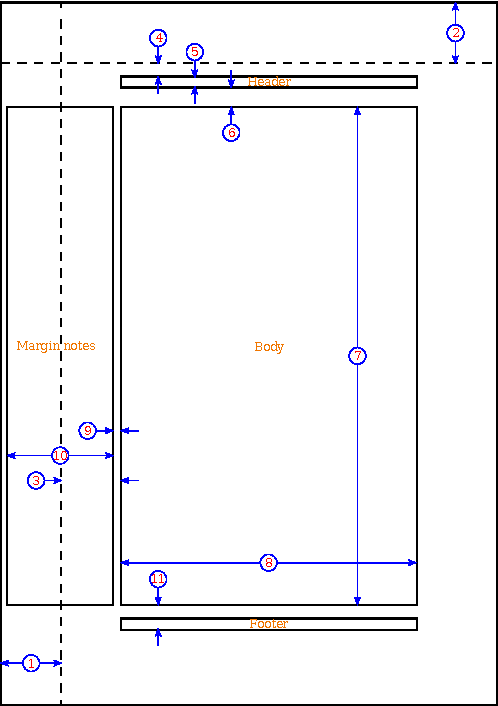
\includegraphics[scale=1.2]{img/page_layout.pdf}
		\end{column}
	\end{columns}
\end{frame}

%\begin{frame}[fragile]
	\frametitle{Theorem-Umgebung}
	\begin{itemize}
		\item der \befehl{newtheorem} Befehl dient der Erzeugung von Umgebungen für Theoreme, Sätze, Definitionen etc.
		\begin{itemize}
			\item \befehl{newtheorem\{name\}\{beschriftung\}}
			\item \befehl{newtheorem\{name\}\{beschriftung\}[zaehler]}
		\end{itemize}
		\begin{center}
			\begin{tabular}{rl}
				\emphkeyword{name} & Name der Theorem-Umgebung\\
				\emphkeyword{beschriftung} & die Bezeichnung der Umgebung im Dokument\\
				\emphkeyword{zaehler} & der Zähler der zur Nummerierung verwendet wird
			\end{tabular}
		\end{center}
	\end{itemize}
\end{frame}

\begin{frame}
	\frametitle{Theorem-Umgebung -- Beispiel}
	
	\latexBeispielDirekt{Theorem-Umgebung -- Beispiel}{examples/Theorem_Umgebung/Theorem_Umgebung}
\end{frame}
%\begin{frame}[fragile]
	\frametitle{Bibliographie}
	\begin{itemize}
        \item \LaTeX{} stellt mit BibTeX ein sehr mächtiges System zur Verwaltung von Literaturverweisen bereit.
		\item Um BibTeX nutzen zu können, muss zunächst eine Datenbank angelegt werden.
		\item Die Datenbank ist eine einfache Textdatei mit Einträgen für die verschiedenen zitierten Quellen.
		\item allgemeiner Aufbau eines Eintrags:
		\begin{itemize}
			\item \keyword{@literaturtyp\{kennung, name1=''Wert1'', name2=''Wert2'', ...\}}
		\end{itemize}
		\begin{center}
			\begin{tabular}{rl}
				\emphkeyword{literaturtyp} & spezifiziert die Art der Quelle\\
				& unterschiedliche Eintragstypen erfordern unterschiedliche\\
				& Angaben zur Quelle \\[0.2cm]
				\emphkeyword{kennung} & damit kann auf den Eintrag referenziert werden\\[0.2cm]
				\emphkeyword{name=''wert''} & Zuweisung von Werten an die verschiedenen Felder
			\end{tabular}
		\end{center}
	\end{itemize}
\end{frame}

\begin{frame}[fragile]
	\frametitle{Bibliographie -- Unterstützte Literatur-Typen}
	\begin{center}
		\begin{tabular}{rl}
			\emphkeyword{article} & Veröffentlichung in einer Zeitschrift\\
			\emphkeyword{book} & Buch\\
			\emphkeyword{booklet} & Buch ohne Verleger\\
			\emphkeyword{inbook} & Teil eines Buches\\
			\emphkeyword{incollection} & Teil einer Buchreihe\\
			\emphkeyword{inproceedings} & Teil einer Veröffentlichung zu einer Konferenz\\
			\emphkeyword{manual} & Technische Dokumentation \\
			\emphkeyword{masterthesis} & Masterarbeit\\
			\emphkeyword{phdthesis} & Doktorarbeit\\
			\emphkeyword{proceedings} & Veröffentlichung zu einer Konferenz\\
			\emphkeyword{techreport} & Technischer Bericht\\
			\emphkeyword{unpublished} & unveröffentlicht\\
			\emphkeyword{misc} & falls alles andere nicht passt
		\end{tabular}
	\end{center}
\end{frame}	

\begin{frame}[fragile]
	\frametitle{Bibliographie -- Unterstützte Felder}
	\vspace{-0.7cm}
	\begin{center}
		\begin{tabular}{rl}
			\emphkeyword{address} & die Adresse des Verlags oder einer anderen Institution\\
			\emphkeyword{annotate} & Anmerkungen \\
			\emphkeyword{author} & Namen der Autoren (in BibTeX Format)\\
			& \tabitem mehrere Namen werden durch \keyword{AND} getrennt \\
			& \tabitem zwei Möglichkeiten Namen zu schreiben:\\
			& ~~~ \keyword{Donald E. Knuth} \textit{oder} \keyword{Knuth, Donald E.}\\
			\emphkeyword{booktitle} & Titel des Buchs \\
			\emphkeyword{chapter} & Kapitel- oder Abschnitt-Nummer\\
			\emphkeyword{crossref} & Datenbank-Schlüssel\\
			\emphkeyword{edition} & Auflage (z. B. eines Buchs)\\
			\emphkeyword{editor} & Namen der Editoren (analog dem \keyword{author}-Feld)\\
			\emphkeyword{howpublished} & Veröffentlichungsart \\
			\emphkeyword{institution} & fördernde Institution eines technischen Reports\\	
			\emphkeyword{journal} & Zeitschriftenname (häufig abgekürzt)
		\end{tabular}
	\end{center}
\end{frame}

\begin{frame}[fragile]
	\frametitle{Bibliographie -- Unterstützte Felder}
	\vspace{-0.7cm}
	\begin{center}
		\begin{tabular}{rl}
            \emphkeyword{key} & Feld zur Sortierung und Erstellung von Labels\\
			\emphkeyword{month} & Monat der Veröffentlichung/Erscheinung\\
			\emphkeyword{note} & zusätzliche Information\\
			\emphkeyword{number} & Nummer einer Zeitschrift, eines Reports oder eines Bandes\\
			\emphkeyword{organization} & fördernde Organisation\\
			\emphkeyword{pages} & Seitenzahlen oder Seitenzahlbereich (z. B. \keyword{7-33})\\
			\emphkeyword{publisher} & Name des Verlags\\
			\emphkeyword{school} & Name der ``Schule'', an der eine Abschlussarbeit geschrieben wurde\\
			\emphkeyword{series} & Name einer Reihe\\
			\emphkeyword{title} & Titel des Werkes\\
			\emphkeyword{type} & Typ eines technischen Reports\\
			\emphkeyword{volume} & Band einer Zeitschrift oder eines Buches\\
			\emphkeyword{year} & Jahr der Veröffentlichung/Erscheinung
		\end{tabular}
	\end{center}
\end{frame}

\begin{frame}[fragile]
	\frametitle{Bibliographie einbinden}
	\begin{itemize}
		\item verschiedene Felder sind bei verschiedenen Literaturtypen vorgeschrieben
		\item es gibt noch weitere Felder wie \keyword{ISBN}, \keyword{doi}, \keyword{abstract}, ...
		\item Sonderzeichen und Umlaute müssen speziell maskiert werden\\[0.5cm]
		\item BibTeX muss eigens aufgerufen werden:\\
		\kommandozeile{latex beispiel}\\
		\kommandozeile{bibtex beispiel}\\
		\kommandozeile{latex beispiel}\\
		\kommandozeile{latex beispiel}
		\item BibTeX prüft die Syntax der Einträge und erzeugt eine Datei, die in das \LaTeX-Dokument eingebunden werden kann
        \item nach Aufruf von BibTeX muss \LaTeX{} die Datei zwei mal kompilieren, damit alle Referenzen korrekt gesetzt werden
	\end{itemize}
\end{frame}

\begin{frame}[fragile]
	\frametitle{Bibliographie einbinden}
	\begin{itemize}
		\item um die Bibliographie anzuzeigen, verwendet man den folgenden Befehl:\\
		\befehl{bibliography\{literatur\}}
		\item \keyword{literatur} bezeichnet dabei die Datei mit den entsprechenden Literaturangaben
		\item aufgelistet werden alle Quellen, die im Dokument zitiert wurden (mittels dem Befehl \befehl{cite\{kennung\}})
		\item durch \befehl{nocite\{kennung\}} wird auch der \keyword{kennung} entsprechende Eintrag aufgeführt, auch wenn er nicht zitiert wurde
		\item die Formatierung hängt von \befehl{bibliographystyle} ab
		\item es gibt verschiedene Pakete zur Gestaltung der Literaturverweise, z. B. \keyword{natbib}
	\end{itemize}
\end{frame}

\begin{frame}[fragile]
	\frametitle{Bibliographie mit \emphkeyword{natbib}}
	\vspace{-1cm}
	\begin{itemize}
		\item \keyword{natbib} wird durch \befehl{usepackage\{natbib\}} (in der Präambel) eingebunden
		\item als Format wird dann \keyword{plainnat} gewählt:
		\befehl{bibliographystyle\{plainnat\}}
		\item \keyword{natbib} unterstützt mehrere zusätzliche Literaturangaben wie
		\begin{center}
			\begin{tabular}{rl}
				\emphkeyword{ISBN} & ISBN-Nummer eines Buches\\
				\emphkeyword{ISSN} & ISSN-Nummer einer Zeitschrift\\
				\emphkeyword{URL} & Internet-Adresse für Online-Dokumente\\
				\emphkeyword{DOI} & Digital Object Identifier
			\end{tabular}
		\end{center}
	\end{itemize}
	
	\begin{columns}[c]
		\begin{column}{0.54\textwidth}
			\begin{block}{Zitieren mit \keyword{natbib}}
			\lstinputlisting{examples/NatBib/NatBib}
			\end{block}
		\end{column}
		\begin{column}{0.44\textwidth}
			\shadowbox{\begin{minipage}{0.99\textwidth} Knuth et al. (1993)\\(Knuth et al., 1993)\\(siehe Knuth et al., 1993, S. 13)\\Knuth et al.\\1993 \end{minipage}}
		\end{column}
	\end{columns}
\end{frame}

%\begin{frame}[fragile]
	\frametitle{\LaTeX\ Beamer}
	\begin{itemize}
		\item Klasse zur Erstellung von Präsentationen mit \LaTeX
		\item Benutzerhandbuch zur Klasse:
		\href{http://ftp.fau.de/ctan/macros/latex/contrib/beamer/doc/beameruserguide.pdf}{http://ftp.fau.de/ctan/macros/latex/contrib/beamer/doc/beameruserguide.pdf} \\[0.5cm]
		\item Grundkonzept: eine \emphkeyword{frame} entspricht einer Seite (Folie)
		\item innerhalb der Frames können (fast alle) normalen \LaTeX-Befehle verwendet werden
	\end{itemize}
\end{frame}

\begin{frame}[fragile]
	\frametitle{\LaTeX\ Beamer -- Präambel}
	\begin{block}{\LaTeX\ Beamer -- Beispiel - Präambel}
		\begin{lstlisting}
\documentclass{beamer}
\usepackage[ngerman]{babel}
\usepackage[utf8]{inputenc}

\usetheme{Luebeck}
\usecolortheme{orchid}
\usefonttheme{default}
\useinnertheme{rounded}
\useoutertheme{shadow}
		\end{lstlisting}
	\end{block}
\end{frame}


\begin{frame}
	\frametitle{\LaTeX\ Beamer -- Hello World}
	\latexBeispielDatei{Hello World Frame}{examples/Beamer_HelloWorld/beamer_helloworld}
\end{frame}

\begin{frame}[fragile]
	\frametitle{\LaTeX\ Beamer -- Frames}
	
	\begin{block}{\LaTeX Beamer -- Frames -- Allgemeine Form}
		\begin{lstlisting}
\begin{frame}[Overlay][Optionen]{Titel}{Untertitel}
  Inhalt
\end {frame}
		\end{lstlisting}
	\end{block}
	\begin{center}
		\begin{tabular}{rl}
			\emphkeyword{Overlay} & \keyword{<+->} sorgt dafür, dass Listen schrittweise aufgebaut werden\\
			\emphkeyword{Optionen} & Anzeigeoptionen für diese Folie (mehrere Optionen müssen\\
			& durch Kommas abgetrennt werden)\\
			\emphkeyword{Titel} & Titel der Folie; kann auch mit \befehl{frametitle} gesetzt werden\\
			\emphkeyword{Untertitel} & Untertitel der Folie; kann auch mit \befehl{framesubtitle}\\
			& gesetzt werden
		\end{tabular}
	\end{center}
\end{frame}

\begin{frame}[fragile]
	\frametitle{\LaTeX\ Beamer -- Frames -- Optionen}
	\begin{center}
		\begin{tabular}{rl}
			\emphkeyword{t} & Ausrichtung des Inhalts oben (\textit{top})\\
			\emphkeyword{c} & Ausrichtung des Inhalts mittig (\textit{center})\\
			\emphkeyword{b} & Ausrichtung des Inhalts unten (\textit{bottom})\\
			\emphkeyword{label=name} & Label für die Folie setzen\\
			\emphkeyword{plain} & Kopf- und Fußzeile unterdrücken\\
			\emphkeyword{squeeze} & Inhalt zusammenrücken\\
			\emphkeyword{fragile} & notwendig für Folien mit Quelltext (\keyword{verbatim})
		\end{tabular}
	\end{center}
\end{frame}

\begin{frame}[fragile]
	\frametitle{\LaTeX\ Beamer -- Blöcke}
	\begin{block}{Block}
		erzeugt durch:
		\begin{lstlisting}
			\begin{block}{Block}
			...
			\end{block}
		\end{lstlisting}
	\end{block}
	\begin{exampleblock}{Beispiel}
		erzeugt durch \keyword{exampleblock}-Umgebung
	\end{exampleblock}
	\begin{alertblock}{Wichtig}
		erzeugt durch \keyword{alertblock}-Umgebung
	\end{alertblock}
	\vfill
	\begin{itemize}
		\item nützlich um thematisch zusammenzufassen
		\item das Aussehen variiert je nach Themenvorlage und eigenen Einstellungen
	\end{itemize}
\end{frame}

\begin{frame}[fragile]
	\frametitle{\LaTeX\ Beamer -- Spalten}
	\vspace{-1cm}
	\begin{columns}
		\column{0.5\textwidth}{
			\begin{block}{Spalte 1}
				...
			\end{block}}
		\column{0.5\textwidth}{\begin{block}{Spalte 2}
				...
			\end{block}}
	\end{columns}
	\vfill
	\begin{block}{Quellcode}
		\begin{lstlisting}
\begin{columns}
  \column{0.5\textwidth}{
    \begin{block}{Spalte 1}
      ...
    \end{block}}
  \column{0.5\textwidth}{
    \begin{block}{Spalte 2}
      ...
    \end{block}}
\end{columns}
		\end{lstlisting}
	\end{block}
	\begin{itemize}
		\item auch mehr als zwei Spalten möglich
	\end{itemize}
\end{frame}

\begin{frame}[fragile]
	\frametitle{\LaTeX\ Beamer -- Overlays}
	\begin{itemize}
		\item Frames können mehrere Overlays enthalten.
		\item Overlays sorgen dann für das stückweise "Aufbauen" einer Folie.
		\item Der \LaTeX-Seitenzähler wird dabei angehalten.
		\item Inhalte können nach und nach Erscheinen oder nur zu bestimmten Zeiten sichtbar sein.
	\end{itemize}
	
	\begin{columns}
		\column{0.5\textwidth}{
			\begin{block}{Quelltext}
				\begin{lstlisting}
Erster Teil
\pause \\
Zweiter Teil
				\end{lstlisting}
			\end{block}}
		\column{0.5\textwidth}{\begin{block}{Vorschau}
				Erster Teil
				\pause \\
				Zweiter Teil
			\end{block}}
	\end{columns}
\end{frame}

\begin{frame}[fragile]
	\frametitle{\LaTeX\ Beamer -- Overlays -- Beispiele Quellcode}
	\begin{block}{Beispiele für Overlay Steuerung}
		\begin{lstlisting}
\begin{itemize}
  \visible<1>{\item Dieser Text erscheint nur auf Overlay 1.}
  {\color<1-3>{red}{\item Dieser Text ist auf Overlays 1 bis 3 rot.}}
  {\color<2->{blue}{\item Dieser Text ist ab Overlay 2 blau.}}
  \only<-3>{\item Dieser Text erscheint nur bis Overlay 3.}
  \textbf<1,3,5>{\item Dieser Text erscheint auf Overlays 1, 3 und 5 im Fettdruck.}
  \alt<2>{\item Dieser Text erscheint nur auf Overlay 2.}{\item Sonst erscheint dieser Text.}
\end{itemize}
		\end{lstlisting}
	\end{block}
\end{frame}

\begin{frame}[fragile]
	\frametitle{\LaTeX\ Beamer -- Overlays -- Beispiele Quellcode}
	\begin{flushright}
		Overlay \only<1>{1}\only<2>{2}\only<3>{3}\only<4>{4}\only<5>{5} / 5
	\end{flushright}
	\begin{itemize}
		\visible<1>{\item Dieser Text erscheint nur auf Overlay 1.}
		{\color<1-3>{red}{\item Dieser Text ist auf Overlays 1 bis 3 rot.}}
		{\color<2->{blue}{\item Dieser Text ist ab Overlay 2 blau.}}
		\only<-3>{\item Dieser Text erscheint nur bis Overlay 3.}
		\textbf<1,3,5>{\item Dieser Text erscheint auf Overlays 1, 3 und 5 im Fettdruck.}
		\alt<2>{\item Dieser Text erscheint nur auf Overlay 2.}{\item Sonst erscheint dieser Text.}
	\end{itemize}
\end{frame}
%\begin{frame}
%	\begin{block}{\huge Aufgabe 10 (Präsentationen)}
%		\input{../exercises/exercises/praesentationen}
%	\end{block}
%\end{frame}


%%%%%%%%%%%%%%%%%%%%%%%%%%%%%%%%%%%%%%%%%%%%%%%%%%%%%%%%%%%%%%%%%%%%%%%%%%%%%
% S C H Ü L E R - V E R S I O N
%%%%%%%%%%%%%%%%%%%%%%%%%%%%%%%%%%%%%%%%%%%%%%%%%%%%%%%%%%%%%%%%%%%%%%%%%%%%%
%\begin{frame}
	\frametitle{Slides and Examples}

        \begin{itemize}
		\item Slides:\\
                  \url{https://depot.tu-dortmund.de/dlep3}
		\item Examples:\\ 
                  \url{https://depot.tu-dortmund.de/5al36} 
        \end{itemize}

\end{frame}

\begin{frame}
	\frametitle{About ParaView}

      \begin{block}{ParaView Features}
        \begin{itemize}
		\item Open-source and multi-platfrom visualization software
		\item Visualization backend provided by VTK library
		\item Huge number of visualization filters  
                \item Extension is possible by programmable filters (Python) or 
                \item User defined plugins  
		\item Import and export of data to various formats used in CFD packages
		\item Easy access to numerical data for internal or external plotting etc.
		\item Tasks can be automated by using the PvPython interface
		\item Client/Server paradigm to view Big Data on remote clusters
        \end{itemize}
      \end{block}

\end{frame}


\begin{frame}
  \frametitle{ParaView Software Ecosystem}
  \vspace{-0.9cm}
  \begin{tikzpicture}[remember picture,overlay]
    \tikzset{shift={(current page.center)},yshift=-1.5cm}

    \node[text width=8cm] (C1) at (-8, -0.0) {
      \begin{block}{VTK}
        \begin{itemize}
          \item Visualization backend
          \item Uses OpenGL
        \end{itemize}
      \end{block}
    };

    \node[text width=8cm] (C2) at (8,-0.7) {
      \begin{block}{Qt (cute)}
        \begin{itemize}
          \item Provides widges and other GUI controls
          \item Support for modular plugins
        \end{itemize}
      \end{block}
    };

    \node[text width=8cm] (C3) at (0,4) {
      \begin{block}{CMake}
        \begin{itemize}
          \item Script language to control the building process
          \item Generates a wide range of specific build files
        \end{itemize}
      \end{block}
    };

    \node[text width=8cm] (C4) at (0,-4.85) {
      \begin{block}{ParaView}
        \begin{itemize}
          \item VTK visualization by GUI
          \item Scripting via Python
          \item Extension by plugins
        \end{itemize}
      \end{block}
    };

\end{tikzpicture}
\end{frame}


\begin{frame}
  \frametitle{Use Cases of Visualization Software}

      \begin{block}{Typical ParaView Use Cases}
        \begin{itemize}
          \item Provide an intuitive illustration of raw simulation data

          \item Highlight key features of specific flow features

          \item Provide an intuitive understanding for non-expert viewers  

          \item Help in the testing/debugging process of CFD software 

          \item Assist during result validation by providing analysis tools  

          \item Convert data in different formats in order to communicate with scientific partners
        \end{itemize}
      \end{block}

\end{frame}

\begin{frame}
  \frametitle{ParaView Interface}

  \begin{tikzpicture}[remember picture,overlay]
    \tikzset{shift={(current page.center)},yshift=-1.5cm}

    \node[align=center,scale=0.3,transform shape] (C1) at (0,0)
    {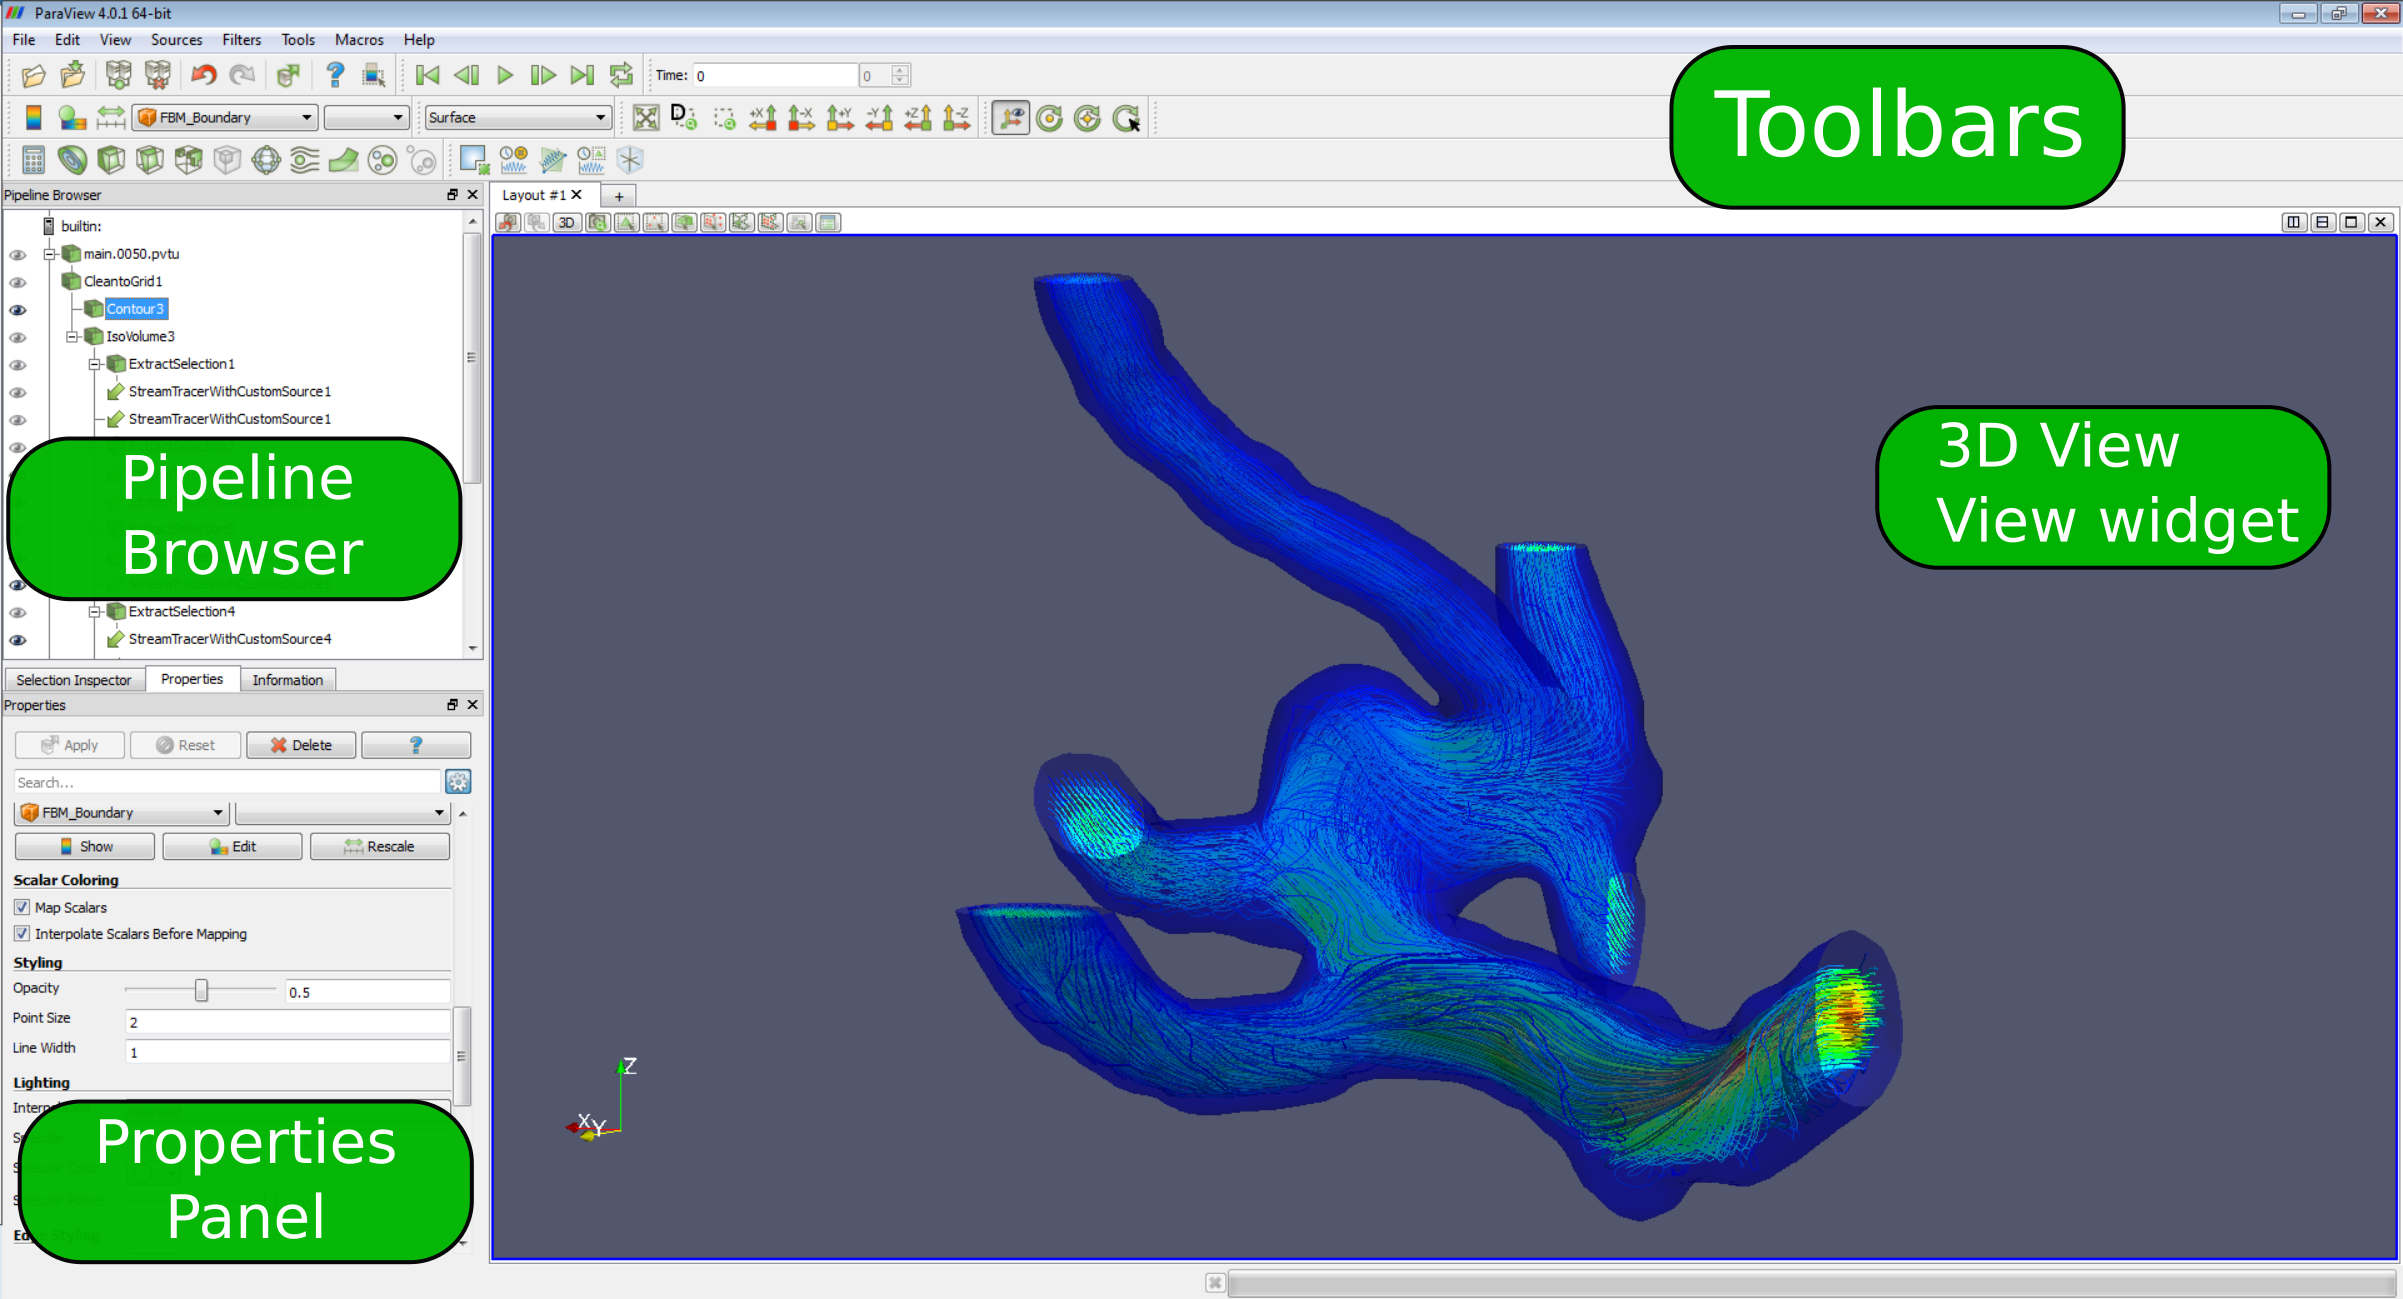
\includegraphics{screenshots/pv-gui.png}};

\end{tikzpicture}

\end{frame}

\begin{frame}[fragile]
  \frametitle{Filter Pipeline Concept}

    \begin{minipage}{0.45 \textwidth}

      \begin{tikzpicture}%[nodes=draw]

    \node[text width=8cm] (C1) at (-8, 1.25) {
      \begin{block}{Filter Pipeline}
        \begin{itemize}
          \item A \keyword{filter} is an operation on an input data set
          \item Filters can be chained (pipelined)  
          \item More complex visualizations require multiple filters 
        \end{itemize}
      \end{block}
    };

    \node[align=center,scale=0.5,transform shape] (C1) at (-10,-5.0)
    {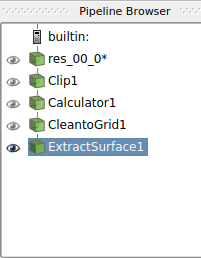
\includegraphics{screenshots/filters.png}};

    \end{tikzpicture}

    \end{minipage}
    \begin{minipage}{0.45 \textwidth}
      \begin{center}
        \begin{tikzpicture}%[nodes=draw]

          \node[align=center,scale=0.189,transform shape] (C1) at (10,-1)
          {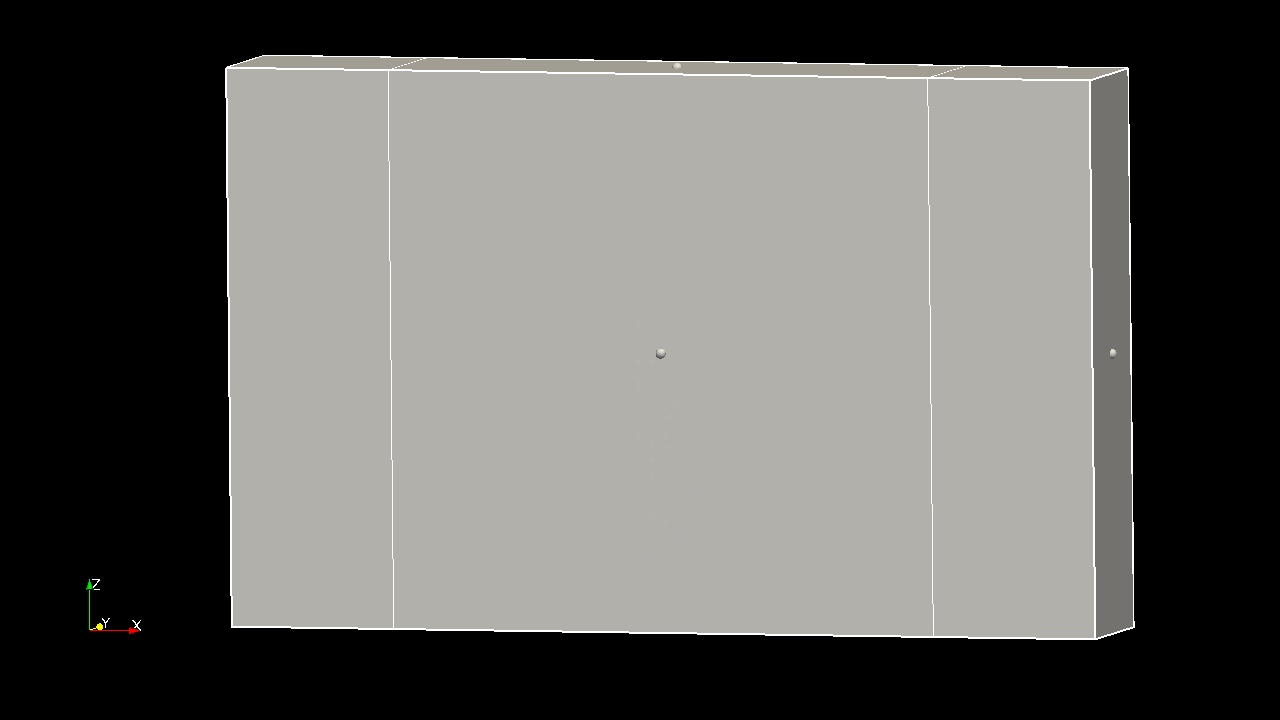
\includegraphics{screenshots/begin-filter.png}};

            \node [scale=2.8,
            fill=TUgreen, 
            single arrow,
            rotate=270, 
            font=\sffamily
            ] at (10.0,-4.22)  
            {\rotatebox{270}{}};

          \node[align=center,scale=0.8,transform shape] (C2) at (10,-8)
          {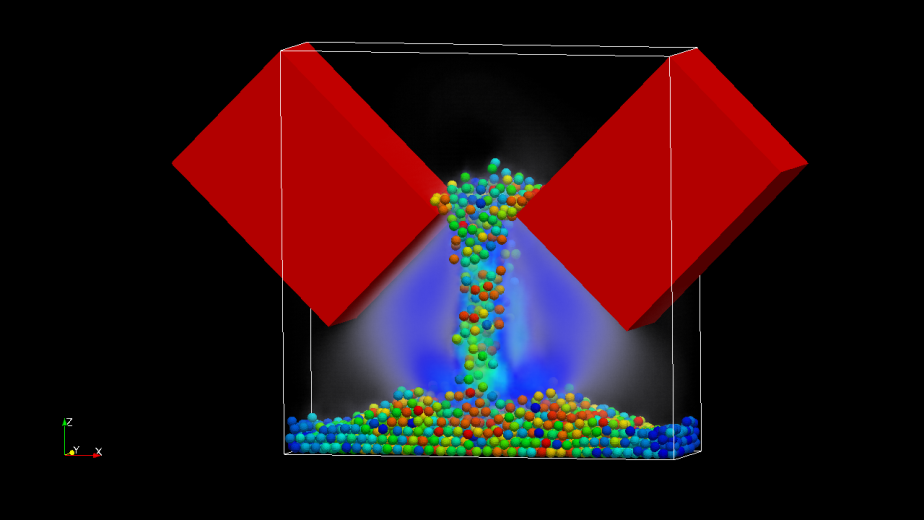
\includegraphics{screenshots/end-filter.png}};

        \end{tikzpicture}
      \end{center}
    \end{minipage}
\end{frame}

\begin{frame}
  \frametitle{Camera and Axes Toolbar}

  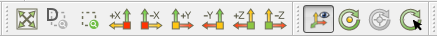
\includegraphics[width=\textwidth]{screenshots/camerabar.png}

    \begin{itemize}
      \item Reset the camera to its default parameters
      \item Magnify a rectangular selection of the view area
      \item Choose a certain coordinate axes plane to look at
      \item Toggle rendering of orientation axes 
      \item Toggle rendering of center of rotation 
      \item Select a new center of rotation 
    \end{itemize}
\end{frame}

\begin{frame}
  \frametitle{Basic Filters}

    \begin{itemize}
      \item \keyword{Slice}: Extract a plane, box-, sphere- or cylinder surface out of a data set
      \item \keyword{Clip}: Extract a plane, box-, sphere- or cylinder volume out of a data set
      \item \keyword{Warp by Scalar}: Visualizes a scalar value by a height extrusion on a 2D data set 
      \item \keyword{Contours}: Increases visibility of different solution contour levels 
      \item \keyword{Surface LIC}: Streamlines on pixel basis, highlights small scale flow features 
      \item \keyword{Glyphs}: Streamlines on pixel basis, highlights small scale flow features 

      \item \keyword{Stream Traces}: Visualizes the pathline of a particle through a \emph{stationary} vector field 
    \end{itemize}

\end{frame}

\begin{frame}
  \frametitle{State Files}

    \begin{itemize}
      \item \keyword{State file}: XML format based file with the ending .pvsm that is used to store the currently applied filters and a reference to the currently loaded data sets to a file
      \item Used to quickly restore a state or to recover from a crash
      \item The reference to the data set can be changed upon loading the state file in order to apply the
        filters to a different data set or if the location of the data on the hard drive has changed
      \item This way state files can be used to exchange a ParaView visualization with collaborators, they only need to set the location of their data set upon loading the state file
      \item State files can be exchanged between different version of ParaView
      \item Accessible from Menu: \keyword{File->Load State...}
    \end{itemize}
        

\end{frame}

\begin{frame}[plain]
  \vspace{3cm}
  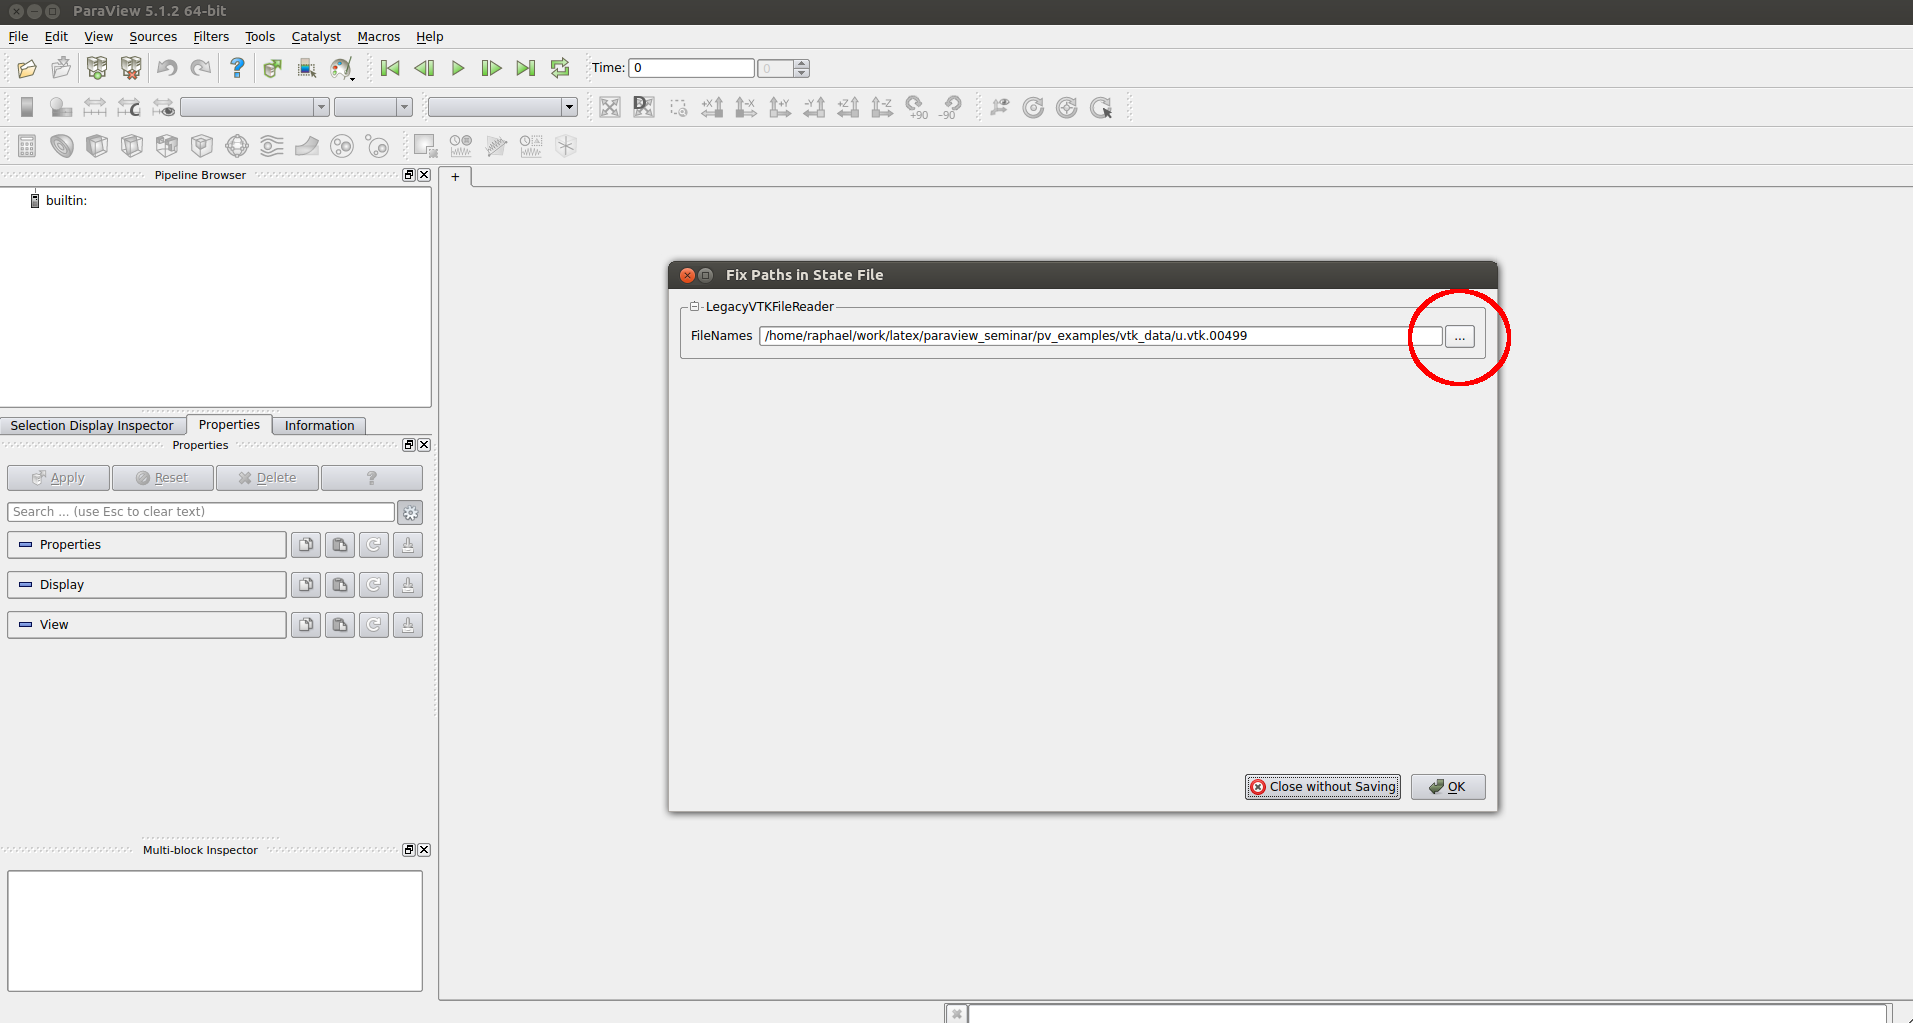
\includegraphics[width=\textwidth]{screenshots/load-state-file.png}
\end{frame}

\begin{frame}
  \frametitle{Examples Files}

    \begin{itemize}
      \item ParaView examples are provided as state files 
      \item Download archive of ParaView examples from:
      \item Extract archive to \kommandozeile{/mypath/to/examples/}
      \kommandozeile{> tar xvfz pv\_examples.tar.gz -C /mypath/to/examples/}
      \item Basic filter examples are located in \kommandozeile{/mypath/to/examples/pv\_examples}
      \item Basic filter examples are located in \kommandozeile{/mypath/to/examples/pv\_examples/BasicFilters}
      \item To load a basic filter example, load the state file and set data path to:
        \kommandozeile{/mypath/to/examples/pv\_examples/vtk\_data/u.vtk}
    \end{itemize}
        

\end{frame}

\begin{frame}
  \frametitle{Basic Filter Gallery I}

    \begin{tikzpicture}%[nodes=draw]

      \node[align=center,scale=0.2,transform shape] (C1) at (0,0)
      {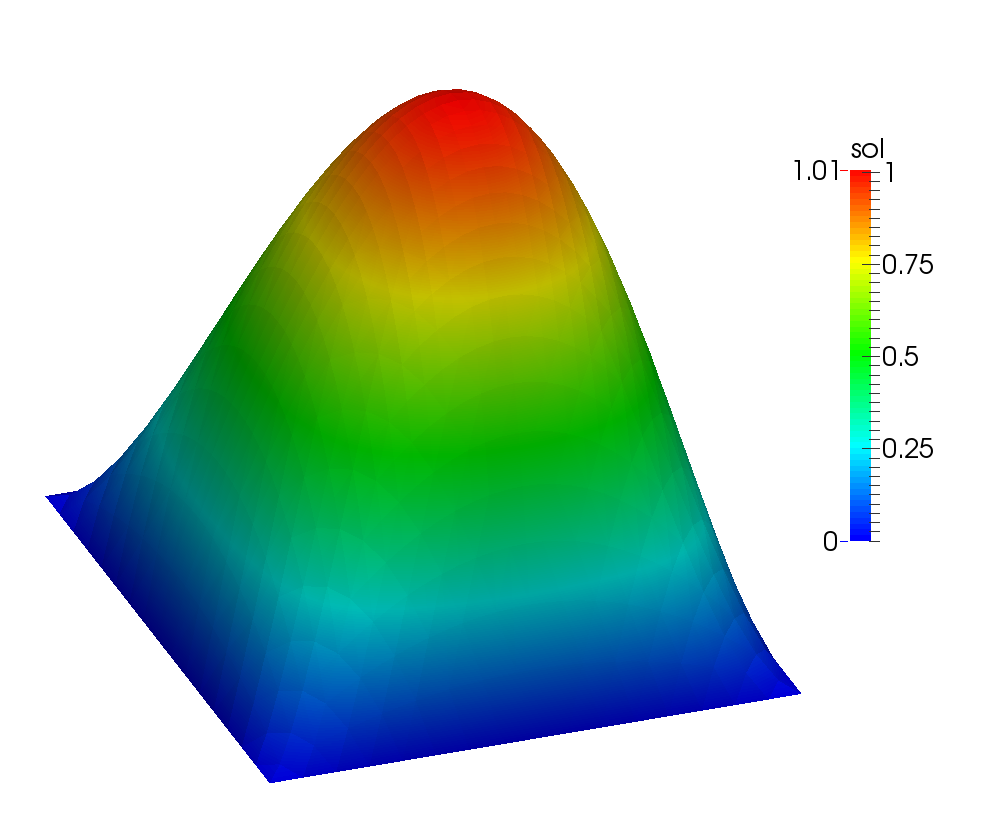
\includegraphics{screenshots/warp-by-scalar.png}};

      \node[align=center,scale=0.2,transform shape] (C2) at (0,-6)
      {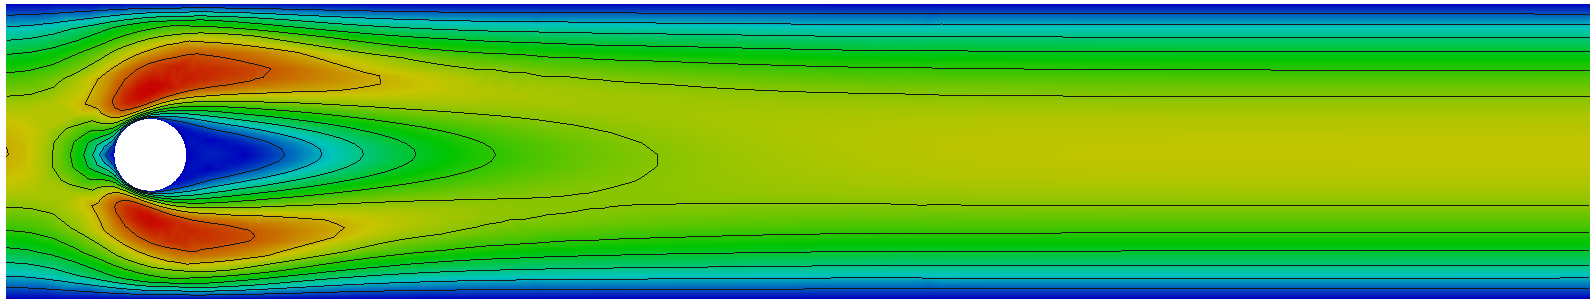
\includegraphics{screenshots/contours.png}};

      \node[align=center,scale=0.2,transform shape] (C3) at (12,-6.05)
      {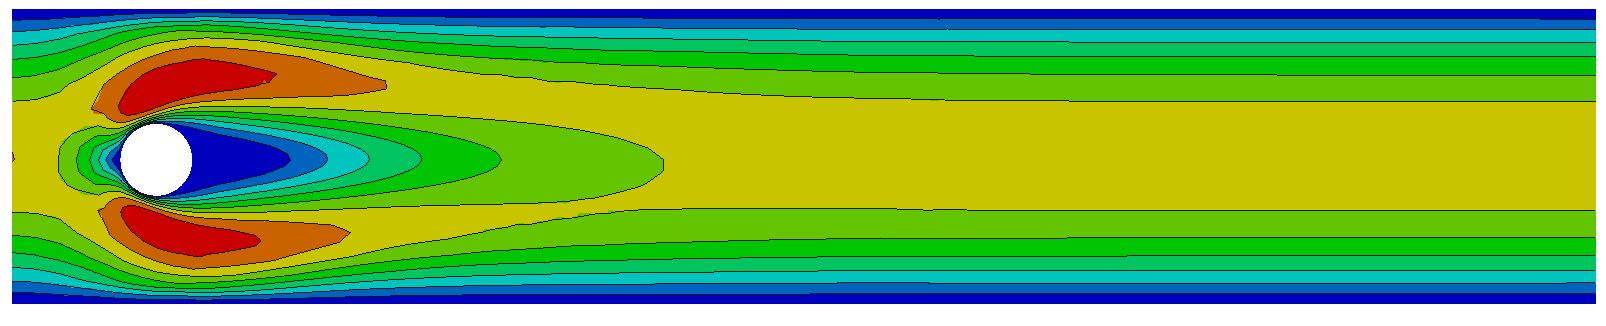
\includegraphics{screenshots/contours_few.png}};

      \node[align=center,scale=0.2,transform shape] (C4) at (12,0)
      {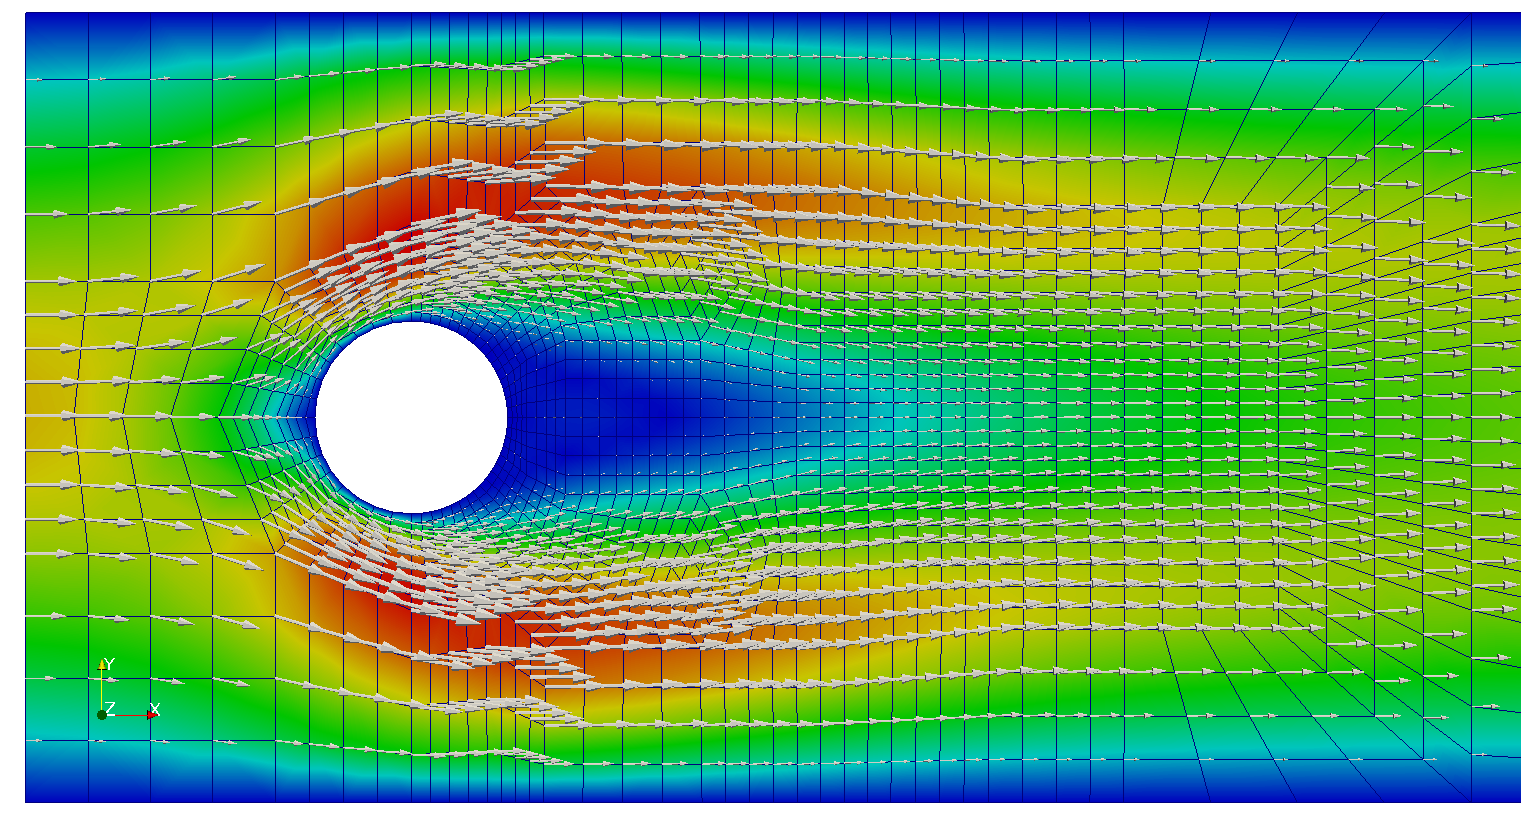
\includegraphics{screenshots/glyphs.png}};

    \end{tikzpicture}

\end{frame}

\begin{frame}

  \frametitle{Basic Filter Gallery II}

    \begin{tikzpicture}%[nodes=draw]

      \node[align=center,scale=0.45,transform shape] (C1) at (0,0)
      {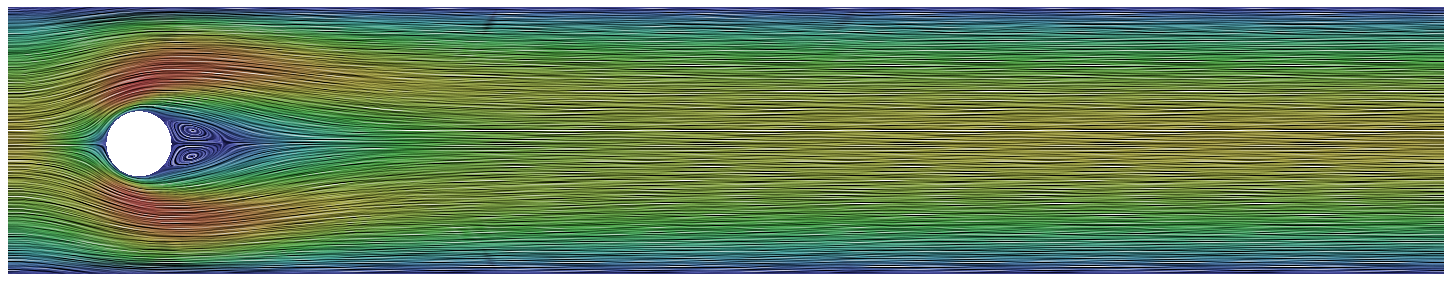
\includegraphics{screenshots/surface_lic_final.png}};

      \node[align=center,scale=0.4,transform shape] (C2) at (0,-6)
      {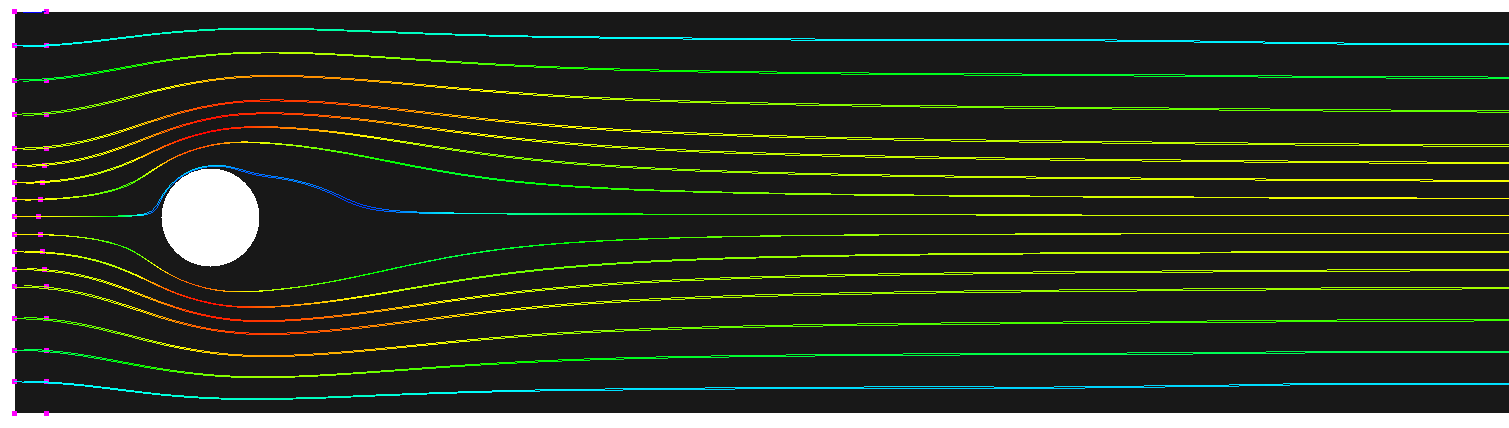
\includegraphics{screenshots/streamlines.png}};


    \end{tikzpicture}

\end{frame}

\begin{frame}

  \frametitle{Configuration of Tracer Filters}

    \begin{itemize}
      \item Tracer type filters need an \keyword{input data set} and a \keyword{seed source}
      \item The input data set is the the flow field  
      \item The seed source is a user-defined starting location for the particles inside the flow field  
    \end{itemize}
    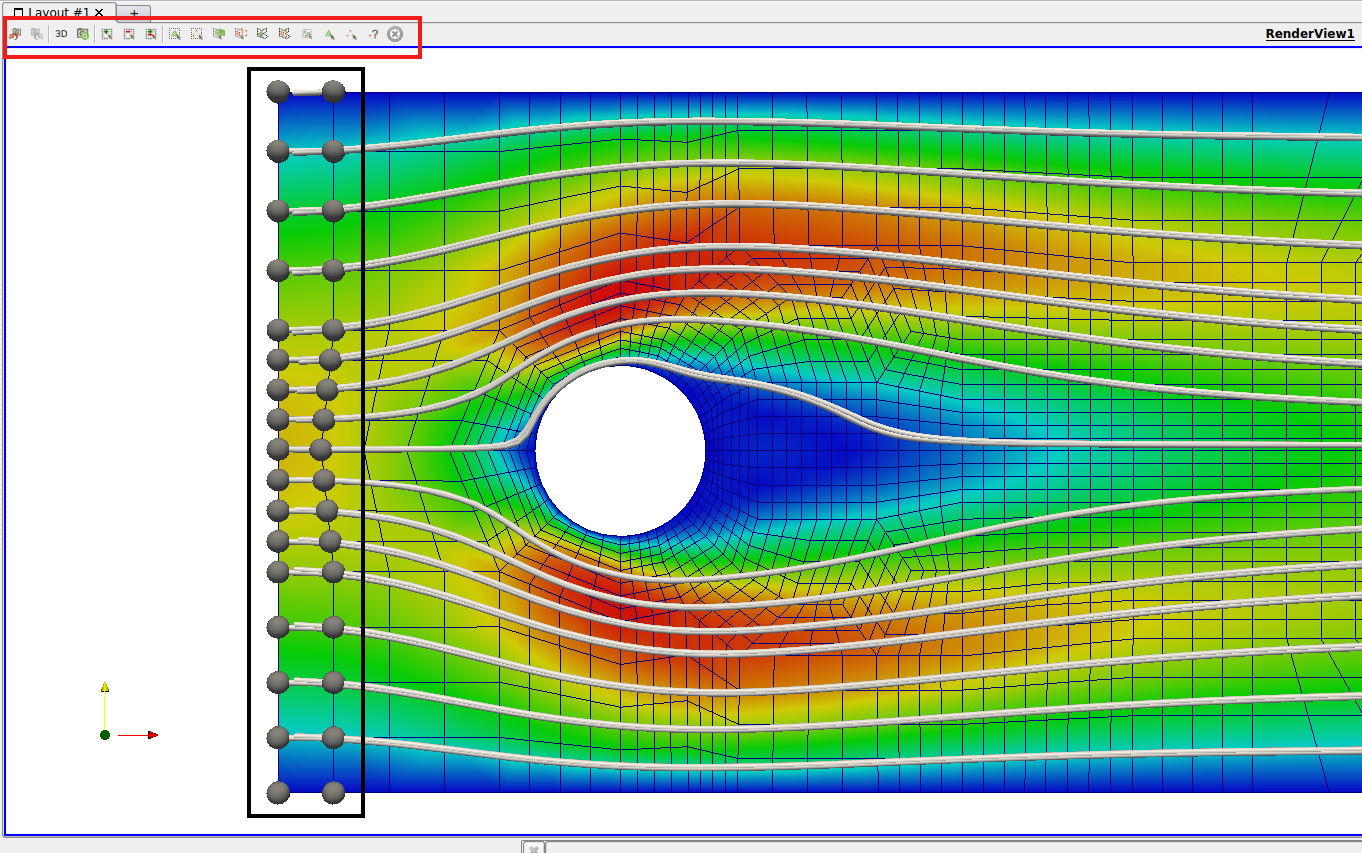
\includegraphics[width=0.5\textwidth]{screenshots/tracer-source.png}

\end{frame}

\begin{frame}

  \frametitle{Advanced Filters: Particle Tracer}

    \begin{itemize}
      \item Used to visualize transient flow data by particles 
      \item A particle path is produced by moving a particle along successive vector fields 
      \item Particle movement can then be animated by the \keyword{Animation Control} 
      \item Particle tracer example location: \kommandozeile{/mypath/to/examples/pv\_examples/AdvancedFilters/particle\_tracer}
    \end{itemize}
    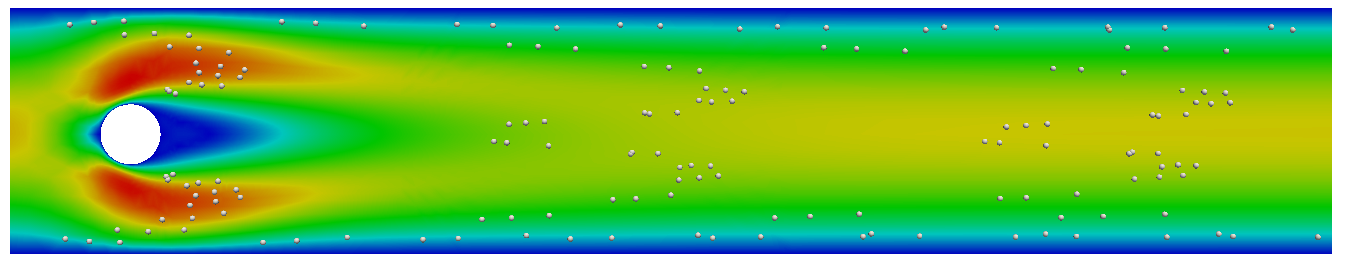
\includegraphics[width=\textwidth]{screenshots/particle-tracer.png}

\end{frame}

\begin{frame}

  \frametitle{List of Useful Filters}

    \begin{itemize}
      \item \keyword{Extract Selection}: Extract a subset from a data set (tracer source, plotting, etc)
      \item \keyword{Extract Surface}: Generates a polygonal surface mesh (exporting, rendering, remeshing) 
      \item \keyword{Clean to Grid}: Removes multiply defined simplices and converts to unstructured mesh
      \item \keyword{Integrate Variables}: Performs numerical integration of the fields defined in the data set on the mesh 
      \item \keyword{Iso-Volume or Iso-Surface}: Constructs a volume or a surface from a function defined on the mesh 
      \item \keyword{Plot Over Line}: Generates a plot of data fields along a line (inflow profiles, etc.) 
      \item \keyword{Calculator}: Use a set of mathematical operations to compute a new data field from existing ones (often used together with integrate variables filter)
    \end{itemize}

\end{frame}

\begin{frame}

  \frametitle{Input Data Formats}

    \begin{itemize}

      \item VTK data formats support polygonal data sets and structured or unstructured meshes 

      \item \keyword{VTK Legacy format .vtk} is a simple format useable for unstructured meshes (not suited for distributed data)  

      \item \keyword{VTK unstructured .vtu} is an xml based format for unstructured meshes   
    \begin{itemize}

      \item Can have the mesh data part encoded in a binary format   

      \item A \keyword{.pvtu} file can be used to reference the partial solutions of a distributed computation   

      \item A \keyword{.pvd} file can be used to add time information   

    \end{itemize}

    \item For further information on VTK file formats see:
      \url{http://www.vtk.org/VTK/img/file-formats.pdf}

  \end{itemize}

\end{frame}

\begin{frame}

  \frametitle{Scripted Postprocessing in ParaView}

  \begin{itemize}

    \item Python interface to access ParaView functionality by scripts

    \item Can be done interactively via a python shell: \keyword{Tools->Python Shell} 

    \item In a 'batch' style by passing a script to the executables \keyword{pvpython} or \keyword{pvbatch} 

    \item Documentation of the ParaView Python interface is under construction at:
      \url{https://www.paraview.org/ParaView3/Doc/Nightly/www/py-doc/}

    \item A trace mechanism is available to generate a PvPython script from a sequence of actions

    \item Beginners should use the trace mechanism (\keyword{Tools->Start Trace}) with the settings \keywords{Show Incremental Trace} and \keywords{only user-modified properties} 

    \item Upon \keyword{Tools->Stop Trace} a file is generated showing the PvPython script equivalent of the user's GUI actions
  \end{itemize}

\end{frame}

\begin{frame}

  \frametitle{PvPython Simple Example}

  \begin{itemize}
      \item PvPython simple example location: \kommandozeile{/mypath/to/examples/pv\_examples/PvPython/paraview\_python}

      \item Navigate to the folder and execute the PvPython script by: \kommandozeile{pvbatch ./python\_test.py \$(pwd)} or for versions higher than 5.1
        \kommandozeile{pvbatch {-}{-}use-offscreen-rendering ./python\_test.py \$(pwd)}

      \item The script will write an image \keyword{res.png} to the directory where you executed it 
      \item \keyword{Exercise:} Try to recreate the python script using the trace mechanism, compare the output images if they are the same.

      \item \keyword{Hint:} Prefer \keyword{pvbatch} over \keyword{pvpython} as pvpython tries to open an X windows which may fail on some computers    
  \end{itemize}

\end{frame}

\begin{frame}

  \frametitle{When to use PvPython}

  \begin{itemize}

    \item Repeated application of filters to a lot of different data sets (parameterize script w.r.t. data set) 

    \item Repeated application of operations that cannot be parametrized by ParaView GUI

    \item Perform an operation that cannot easily be done by ParaView filters 

    \item Quickly and repeatedly generate an ouput of a running simulation 

    \item Generate outputs on remote clusters 

    \item \keyword{ParaView Programmable Filter} or \keyword{Python Calculator} may serve as an alternative 

  \end{itemize}

\end{frame}

\begin{frame}

  \frametitle{Plotting with ParaView}

  \begin{itemize}

      \item PV plotting example: \kommandozeile{/mypath/to/examples/pv\_examples/Plotting/plotting.pvsm}

      \item Common ParaView plotting filters:
      \begin{itemize}

        \item \keyword{Plot Data} 

        \item \keyword{Plot Over Line} 

        \item \keyword{Plot Selection Over Time} 

      \end{itemize}

    \item Data can be exported to .csv to use in your favorite plot generator \keyword{File->Save Data}

    \item ParaView will by default export ALL data fields to the .csv file (even those that you do not want or need for the plot) 

    \item \keyword{Solution 1:} use <awk> to select the data columns you want: \kommandozeile{awk -F \textquotesingle,\textquotesingle $\;$  \textquotesingle\{print \$1 " " \$4\}\textquotesingle} (extract first and fourth column)

    \item \keyword{Solution 2:} Remove unneccessary fields before export: \kommandozeile{/mypath/to/examples/pv\_examples/Plotting/plotting2.pvsm}

  \end{itemize}

\end{frame}

\begin{frame}
  \frametitle{Client-Server Mode}

    \begin{itemize}
      \item In default mode ParaView is both the client and the server
      \item When client/server are different rendering and data processing can
        be handled by different computers 
      \item Simple X forwarding works adequately only if the network speed is fast
      \item Client-Server is preferable to access data on remote (non-local) clusters 
      \item Client-Server steps: \keyword{port forwarding}, \keyword{starting the remote server}, \keyword{connecting the client to the server}  
    \end{itemize}

    \begin{block}{Port Forwarding}
        \begin{itemize}
          \item Establish an ssh tunnel to forward the local port to the remote server: \\  
          \kommandozeile{> ssh lidong1.itmc.tu-dortmund.de \textbackslash}
          \kommandozeile{-L 11111:lidong1.itmc.tu-dortmund.de:11111}
        \end{itemize}
    \end{block}

\end{frame}

\begin{frame}
  %\frametitle{Client-Server Mode II}

    \begin{block}{Start the remote Server}
        \begin{itemize}
          \item Start a ParaView data server on the remote machine  
            \kommandozeile{> pvserver {-}{-}server-port=11111 {-}{-}use-offscreen-rendering}
        \end{itemize}
    \end{block}

    \begin{block}{Connect to the remote Server}
        \begin{itemize}
          \item Start a ParaView client locally  
          \item Press the <Connect> button on the toolbar  
          \item Manually configure the Server dialog:
          \begin{itemize}
            \item Name: myname   
            \item Server Type: Client/Server  
            \item Host: localhost 
            \item Port: 11111 
          \end{itemize}
        \end{itemize}
    \end{block}
  Pitfalls:
    \begin{itemize}
      \item You \textbf{have to} make use the same ParaView version of the client and the server
      \item Check that the port is not occupied, otherwise use a different port: 
      \kommandozeile{> lsof -i:11111}
    \end{itemize}

\end{frame}

\begin{frame}

  \frametitle{Additional ParaView Resources}

  \begin{itemize}
      \item ParaView documentation:\\
        \url{https://www.paraview.org/documentation/}
      \item ParaView Wiki:\\
        \url{https://www.paraview.org/Wiki/ParaView}
      \item ParaView Tutorial:\\
        \url{https://www.paraview.org/Wiki/The\_ParaView\_Tutorial}
      \item ParaView Mailing List:\\
        \url{https://public.kitware.com/mailman/listinfo/paraview}
      \item ParaView Catalyst:\\
        \url{https://www.paraview.org/Wiki/ParaView/Catalyst/Overview}
      \item ParaView Web JavaScript:\\
        \url{www.paraview.org/Wiki/ParaViewWeb\_JavaScript\_Introduction}
  \end{itemize}

\end{frame}


%\begin{frame}
	\frametitle{Spezielle Zeichen}
	\begin{itemize}
		\item bei Verwendung des ASCII-Zeichensatzes: Buchstaben ohne Umlaute, Zahlen und einige Sonderzeichen
		\item manche Zeichen sind \LaTeX-Steuerzeichen und daher reserviert (\$, \_, \{, \},\textbackslash )
        \item solche Sonderzeichen können durch \textbackslash{} maskiert werden: \\[0.5cm]
		\begin{center}
			\begin{tabular}{|cc|cc|} \hline
				\$ & \textbackslash\$ & \% & \textbackslash\% \\
				\{ & \textbackslash\{ & \} & \textbackslash\} \\
				\# & \textbackslash\# & \_ & \textbackslash\_ \\
				\& & \textbackslash\& & & \\ \hline
			\end{tabular}
		\end{center}
	\end{itemize}
\end{frame}

\begin{frame}[fragile]
	\frametitle{Deutsche Texte - Sprachpakete}
    Ohne weitere Angaben nimmt \LaTeX{} an, dass der eingegebene Text in englischer Sprache ist. Daher muss ggf. ein zusätzliches Sprachpaket eingebunden werden:
	\begin{center}
		\begin{block}{Beispiel-Header: deutsches Sprachpaket}
			\begin{lstlisting}
\documentclass[a4paper]{article}      % DIN-A4 Papierformat
\usepackage[ngerman]{babel}           % deutsche Benennung
\usepackage[utf8]{inputenc}
\begin{document}
  ...
\end{document}
			\end{lstlisting}
		\end{block}
	\end{center} \vspace{-1cm}
	\begin{itemize}
		\item \keyword{babel} sorgt für Unterstützung anderer Sprachen (Formate, Umlaute, Benennungen, Silbentrennung)
		\item \keyword{inputenc} unterstützt die direkte Eingabe von Zeichen über die Tastatur
	\end{itemize}
\end{frame}


\begin{frame}[fragile]
	\frametitle{Deutsche Texte -- Umlaute und Anführungszeichen}
	
	Eingabe deutscher Texte:
	\begin{itemize}
		\item Umlaute: \befehl{"a}, \befehl{"o}, \befehl{"u}, \befehl{ss} für ä, ö, ü, ß
		\item Anführungszeichen: \befehl{glq}, \befehl{grq} bzw. \befehl{glqq}, \befehl{grqq} für \glq einfache\grq~ bzw. \glqq doppelte\grqq~ Anführungszeichen
	\end{itemize}
	\vfill
	
	\latexBeispielDirekt{Beispiel: deutsche Umlaute}{examples/Deutsche_Umlaute/Deutsche_Umlaute}
	\vfill
\end{frame}

\begin{frame}[fragile]
	\frametitle{Deutsche Texte - Silbentrennung}
	\begin{itemize}
		\item erfolgt automatisch
		\item mögliche Trennstellen können  durch \befehl{-} auch angegeben werden, z. B.\\
		\lstinline$Donau\-dampf\-schiff\-fahrts\-gesell\-schaft$\\
		oder für das gesamte Dokument in der Präambel:
		\lstinline$\hypenation{Donau\-dampf\-schiff\-fahrts\-gesell\-schaft}$
	\end{itemize}

\end{frame}

%\begin{frame}[fragile]
	\frametitle{Textformatierung -- Schriftstil}
	
	\begin{center}
		\begin{tabular}{l|ll|l}
			Familie & \multicolumn{2}{c|}{Befehle} & Beispiel \\ \hline
			normal (mit Serifen) & \befehl{rmfamily} & \befehl{textr} & \textrm{normal} \\
			serifenfrei & \befehl{sffamily} & \befehl{textsf} & \textsf{serifenfrei} \\
			Schreibmaschine & \befehl{ttfamily} & \befehl{texttt} & \texttt{Schreibmaschine} \\
		\multicolumn{4}{c}{~} \\
			Varianten & \multicolumn{2}{c|}{Befehle} & Beispiel \\ \hline
			aufrecht & \befehl{upshape} & \befehl{textup} & \textup{aufrecht} \\
			italic & \befehl{itshape} & \befehl{textit} & \textit{italic}\\
			Kapitälchen & \befehl{scshape} & \befehl{textsc} & \textsc{Kapitälchen}\\
			fett & \befehl{bfseries} & \befehl{textbf} & \textbf{fett}\\
			unterstrichen & ~ & \befehl{underline} & \underline{unterstrichen}
		\end{tabular}
	\end{center}
\end{frame}

\begin{frame}[fragile]
	\frametitle{Textformatierung -- Schriftgröße}
	\begin{center}
		\begin{tabular}{ll}
		\befehl{tiny} & \tiny{winzig} \\
		\befehl{small} & \small{klein} \\
		\befehl{footnotesize} & {\fontsize{14}{14}\selectfont{}Fußnotengröße}\\
		\befehl{normalsize} & normale Größe\\
		\befehl{large} & {\fontsize{25}{25}\selectfont{}groß} \\
		\befehl{Large} & {\fontsize{30}{30}\selectfont{}größer} \\
		\befehl{huge} & {\fontsize{40}{40}\selectfont{}riesig} \\
		\befehl{Huge} & {\fontsize{50}{50}\selectfont{}Riesig}
		\end{tabular}
	\end{center}
	\vfill
	\begin{itemize}
		\item für einige Wörter: \lstinline${\huge riesig}$
		\item für ganze Absätze: \lstinline$\begin{tiny} ... \end{tiny}$
		\item alternativ: punktgenau durch \lstinline${\fontsize{40}{48}\selectfont{}Test}$\\
		das erste Argument gibt die Schriftgröße an, das zweite den Grundlinienabstand
	\end{itemize}
\end{frame}



%\begin{frame}[fragile]
	\frametitle{Aufzählungen}
	\vspace{-0.5cm}
	drei Grundarten von Aufzählungen: \\
	\begin{tabular}{rl}
		\emphkeyword{itemize} & einfache Aufzählung\\
		\emphkeyword{enumerate} & nummerierte Aufzählung\\
		\emphkeyword{description} & Beschreibung
	\end{tabular}\par \vfill
	
	\begin{columns}[T]
		\begin{column}{0.31\textwidth}
			\begin{block}{\tt\bfseries itemize}
				\begin{itemize}
					\item A \item B \item C
				\end{itemize} 
				\begin{lstlisting}
\begin{itemize}
  \item A
  \item B
  \item C
\end{itemize}
				\end{lstlisting}
			\end{block}
		\end{column}
		\begin{column}{0.31\textwidth}
			\begin{block}{\tt\bfseries enumerate}
				\begin{enumerate}
					\item A \item B \item C
				\end{enumerate} 
				\begin{lstlisting}
\begin{enumerate}
  \item A
  \item B
  \item C
\end{enumerate}
				\end{lstlisting}
			\end{block}
		\end{column}
		\begin{column}{0.31\textwidth}
			\begin{block}{\tt\bfseries description}
				\begin{description}
					\item[A] \ldots \item[B] \ldots \item[C] \ldots
				\end{description} 
				\begin{lstlisting}
\begin{description}
  \item[A] \ldots
  \item[B] \ldots
  \item[C] \ldots
\end{description}
				\end{lstlisting}
			\end{block}
		\end{column}
	\end{columns}
\end{frame}

\begin{frame}[fragile]
	\frametitle{Verschachtelte Aufzählungen}
	\vspace{-0.9cm}
	\latexBeispielDirekt{Beispiel: verschachtelte Aufzählung}{examples/Verschachtelte_Aufzaehlung/Verschachtelte_Aufzaehlung}
\end{frame}
%
\begin{frame}[fragile]
	\frametitle{Mathematik -- Formeln im Fließtext}
	\begin{itemize}
        \item Formeln müssen in \LaTeX{} markiert werden, damit sie korrekt interpretiert werden
		\item im Mathematik-Modus werden Leerzeichen ignoriert und Buchstabenketten als einzelne Zeichen betrachtet
	\end{itemize}
	\vfill
	\latexBeispielDirekt{Beispiel: Formeln im Fließtext}{examples/Formeln_im_Fliesstext/Formeln_im_Fliesstext}
\end{frame}

\begin{frame}[fragile]
	\frametitle{Mathematik -- Formeln in eigenem Absatz}
	\begin{itemize}
		\item soll eine Formel abgesetzt dargestellt werden, so benutzt man die \keyword{displaymath}-Umgebung oder die Kurzschreibweise \lstinline$\[...\]$
	\end{itemize}
	\vfill
	\latexBeispielDirekt{Beispiel: Formeln in eigenem Absatz}{examples/Formeln_eigener_Absatz/Formeln_eigener_Absatz}
\end{frame}

\begin{frame}[fragile]
	\frametitle{Mathematik -- nummerierte Gleichungen}
	\begin{itemize}
		\item Gleichungen können mit der \keyword{equation}-Umgebung automatisch fortlaufend nummeriert werden
		\item mittels der \keyword{align}-Umgebung können mehrzeilige Formeln nummeriert und ausgerichtet werden
		\item \befehl{nonumber} unterdrückt in der \keyword{align}-Umgebung die Nummerierung einer Zeile
	\end{itemize}
	\vfill
	\latexBeispielDirektKlein{Beispiel: mehrzeilige Gleichungen}{examples/Formeln_mehrzeilig/Formeln_mehrzeilig}
\end{frame}


\begin{frame}
  \frametitle{Happy ParaViewing}

    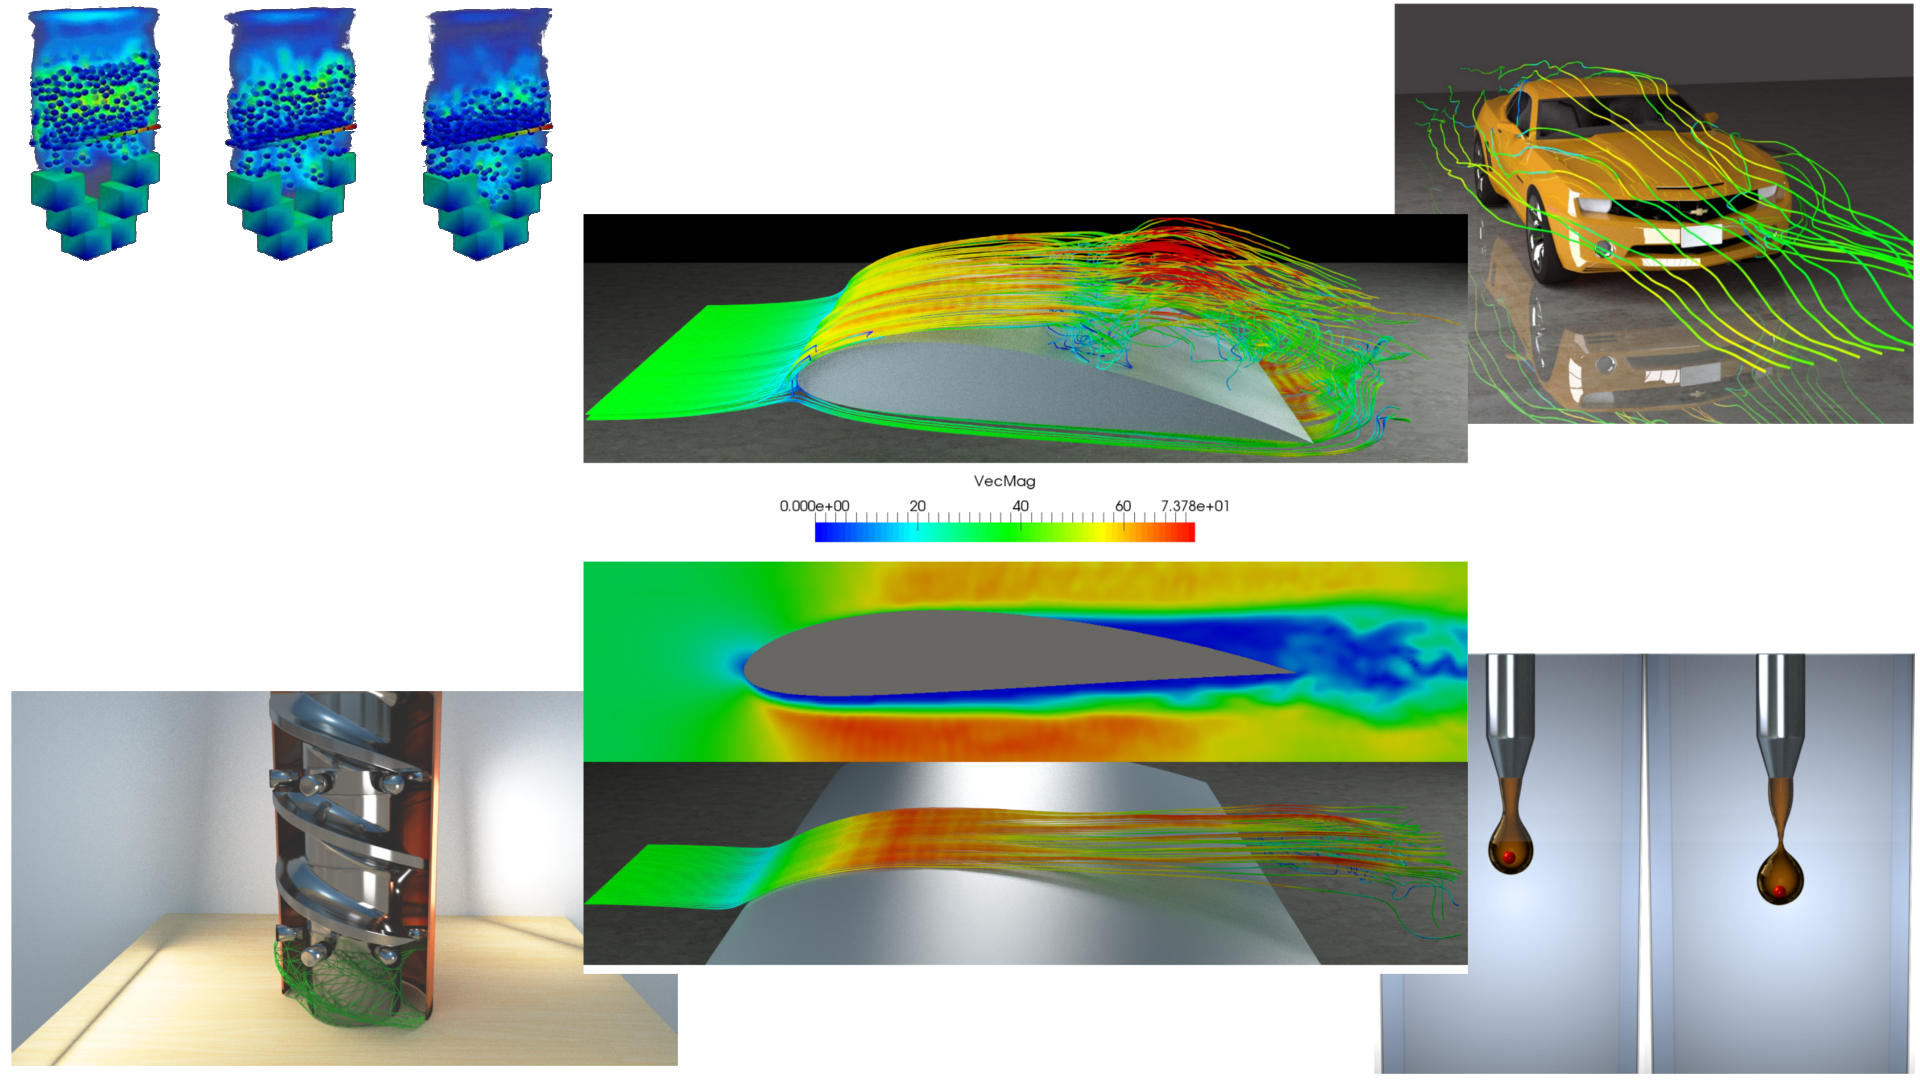
\includegraphics[width=0.9\textwidth]{screenshots/paraviewing.png}

\end{frame}

\end{document}
